% safe参数解决与\!在内的多个冲突
% \sups命令可能被重定义,xeCJK放在tipa后
\RequirePackage[safe]{tipa}

\documentclass[a4paper, zihao=-4, linespread=1]{ctexrep}
\renewcommand{\CTEXthechapter}{\thechapter}
% 最小行间间距设定
\setlength{\lineskiplimit}{3pt}
\setlength{\lineskip}{3pt}

% 中文支持
\setCJKmainfont[BoldFont=SourceHanSerifCN-Bold.otf]{SourceHanSerifCN-Regular.otf} 
  \xeCJKsetup{CJKmath=true}
  \setCJKmathfont{KaiTi}  % 数学环境中使用楷体
\newCJKfontfamily[zhxinwei]\xinwei{STXinwei} % 定义新字体

% 颜色
\usepackage[table]{xcolor}
  \newcommand{\scol}[1]{\colorbox{#1}{\rule{0em}{1ex}}\,#1}
  
% 首字下沉
\usepackage{lettrine}

% 分栏
\usepackage{multicol}
  \setlength{\columnsep}{20pt}
  \setlength{\columnseprule}{0.4pt}

% 数学环境
\usepackage{mathdots} % 数学省略号,会重定义 dddot 和 ddddot
\usepackage{amsmath}  
  \newcommand{\ue}{\mathrm{e}}
  \newcommand{\ud}{\mathop{}\negthinspace\mathrm{d}} % 微分号
\usepackage{amssymb}
\usepackage{mathrsfs} % 线性代数字体
% overline的替代命令
\newcommand{\closure}[2][3]{{}\mkern#1mu\overline{\mkern-#1mu#2}}
\usepackage{yhmath} % \wideparen命令:弧AB
\usepackage{mathtools} % dcases环境,prescript命令
\usepackage{amsthm} % 定理环境
  \theoremstyle{definition}\newtheorem{laws}{Law}[section]
  \theoremstyle{plain}\newtheorem{ju}[laws]{Jury}
  \theoremstyle{remark}\newtheorem*{marg}{Margaret}
\usepackage{esint} % 多重积分,需放在amsmath后
% 箭头与长等号
\usepackage{extarrows}
% 中括号的类二项式命令
\newcommand{\Bfrac}[2]{\genfrac{[}{]}{0pt}{}{#1}{#2}}

% 下划线宏包
\usepackage[normalem]{ulem}
% LaTeX符号宏包
\usepackage{hologo}
	\newcommand{\xelatex}{\Hologo{XeLaTeX}}
	\newcommand{\bibtex}{\Hologo{BibTeX}}
	\newcommand{\tikzz}{Ti\textit{k}Z}
	\newcommand{\bz}{B\'ezier}
% 其他符号
\usepackage{wasysym}
% 带箱小页
\usepackage{boxedminipage}
% 绘图
\usepackage{tikz}
  \usetikzlibrary{calc,intersections,positioning,angles,quotes,decorations.pathmorphing,fit,backgrounds,through}
  \newcommand{\tikzline}[1]{{#1\tikz{\draw[#1,line width=9](0,0)--(0.5,0);}}, }
% 最后一页
\usepackage{lastpage}

% 奇怪的小定义
\newcommand{\dpar}{\\ \mbox{}}  % 空两行
\newcommand{\qd}[1]{{\bfseries{#1}}}  % 强调
\newcommand{\co}[1]{{\bfseries{#1}}}  % Style of concept
\newcommand{\RED}[1]{{\color{cyan}{#1}}}
\newcommand{\cmmd}[1]{\fbox{\texttt{\char92{}#1}}}
\newcommand{\charef}[1]{第\ref{#1}章}
\newcommand{\secref}[1]{第\ref{#1}节}
\newcommand{\pref}[1]{第\pageref{#1}页}
\newcommand{\fref}[1]{图\ref{#1}}
\newcommand{\tref}[1]{表\ref{#1}}

% Quote 环境
\newenvironment{QuoteEnv}[2][]
    {\newcommand\Qauthor{#1}\newcommand\Qref{#2}}
    {\medskip\begin{flushright}\small ——~\Qauthor\\
    \emph{\Qref}\end{flushright}}
% 字体调用
\newcommand{\myfont}[2]{{\fontfamily{#1}\selectfont #2}}

% 编号列表宏包,并自定义了三个列表
\usepackage[inline]{enumitem}
	\setlist[enumerate]{font=\bfseries,itemsep=0pt}
	\setlist[itemize]{font=\bfseries,leftmargin=\parindent}
	\setlist[description]{font=\bfseries\uline}

\newenvironment{fead}{	
    \begin{description}[font=\bfseries\uline,labelindent=\parindent,itemsep=0pt,parsep=0pt,topsep=0pt,partopsep=0pt]}
	{\end{description}}
% 带宽度的
\newenvironment{para}{
	\begin{description}[font=\bfseries\ttfamily,itemsep=0pt,parsep=0pt,topsep=0pt,partopsep=0pt]}
	{\end{description}}
\newenvironment{feae}{
	\begin{enumerate}[font=\bfseries,labelindent=0pt,itemsep=0pt,parsep=0pt,topsep=0pt,partopsep=0pt]}
	{\end{enumerate}}
\newenvironment{feai}{
	\begin{itemize}[font=\bfseries,itemsep=0pt,parsep=0pt,topsep=0pt,partopsep=0pt]}
	{\end{itemize}}
\newenvironment{inlinee}
{\begin{enumerate*}[label=(\arabic*), font=\rmfamily, before=\unskip{:},itemjoin={{;}},itemjoin*={{,以及:}}]}
	{\end{enumerate*}。}

% 目录和章节样式
\usepackage{titlesec}
\usepackage{titletoc}   % 用于目录

\titlecontents{chapter}[1.5em]{}{\contentslabel{1.5em}}{\hspace*{-2em}}{\hfill\contentspage}
\titlecontents{section}[3.3em]{}{\contentslabel{1.8em}}
	{\hspace*{-2.3em}}{\titlerule*[8pt]{$\cdot$}\contentspage}
\titlecontents*{subsection}[2.5em]{\small}{\thecontentslabel{} }{}{, \thecontentspage}[;\qquad][.]
% 章节样式
\setcounter{secnumdepth}{3} % 一直到subsubsection
\newcommand{\chaformat}[1]{%
	\parbox[b]{.5\textwidth}{\hfill\bfseries #1}%
	\quad\rule[-12pt]{2pt}{70pt}\quad
	{\fontsize{60}{60}\selectfont\thechapter}}
\titleformat{\chapter}[block]{\hfill\LARGE\sffamily}{}{0pt}{\chaformat}[\vspace{2.5pc}\normalsize
	\startcontents\setlength{\lineskiplimit}{0pt}\printcontents{}{1}{\setcounter{tocdepth}{2}\songti}]
\titleformat*{\section}{\centering\Large\bfseries}
\titleformat{\subsubsection}[hang]{\bfseries\large}{\rule{1.5ex}{1.5ex}}{0.5em}{}
% 扩展章节
\newcommand{\starsec}{\noindent\fbox{\S\textit{注意:本章节是一个扩展阅读章节。}}
	\\ \mbox{}}

\renewcommand{\contentsname}{目录}
	\renewcommand{\tablename}{表}
	\renewcommand\arraystretch{1.2}	% 表格行距
	\renewcommand{\figurename}{图}
% 设置不需要浮动体的表格和图像标题
\setlength{\abovecaptionskip}{5pt}
\setlength{\belowcaptionskip}{3pt}
\makeatletter
\newcommand\figcaption{\def\@captype{figure}\caption}
\newcommand\tabcaption{\def\@captype{table}\caption}
\makeatother
% 图表
\usepackage{array,multirow,makecell}
  \setlength\extrarowheight{2pt} % 行高增加
\usepackage{diagbox}
\usepackage{longtable}
\usepackage{graphicx,wrapfig}
  \graphicspath{{./tikz/}}
\usepackage{animate}
\usepackage{caption,subcaption}
  \captionsetup[sub]{labelformat=simple}
  \renewcommand{\thesubtable}{(\alph{subtable})}
% 三线表
\usepackage{booktabs}  

% 页面修正宏包
\usepackage{geometry}
  \geometry{vmargin = 1in}

% 代码环境
\usepackage{listings}
% 复制代码时不复制行号
\usepackage{accsupp}
	\newcommand{\emptyaccsupp}[1]{\BeginAccSupp{ActualText={}}#1\EndAccSupp{}}
\usepackage{tcolorbox}
  \tcbuselibrary{listings,skins,breakable,xparse}

% global style
\lstset{
  basicstyle=\small\ttfamily,
  % Word styles
  keywordstyle=\color{blue},
  commentstyle=\color{green!50!black},
  columns=fullflexible,  % Avoid too sparse word spaces
  keepspaces=true,
  % Numbering
  numbers=left,
  numberstyle=\tiny\color{red!75!black}\emptyaccsupp,
  % Lines and Skips
  aboveskip=0pt plus 6pt,
  belowskip=0pt plus 6pt,
  breaklines=true,
  breakatwhitespace=true,
  emptylines=1,  % Avoid >1 consecutive empty lines
  escapeinside=``
}

% TikZ Language Hint
\lstdefinelanguage{tikzlang}{
  sensitive=true,
  morecomment=[n]{[}{]}, % nested comment
  morekeywords={
    draw,clip,filldraw,path,node,coordinate,foreach,pic,
    tikzset
  }
}

% 对于 tcolorbox 中 listings 库的 ''tcblatex'' style 的重现,
% 添加了新的关键词
\lstdefinestyle{latexcn}{
  language=[LaTeX]TeX,
  % More Keywords
  classoffset=0,
  texcsstyle=*\color{blue},
  moretexcs={
    % LaTeX extension
    chapter,section,subsection,setlength,
    thechapter,thesection,thesubsection,theequation,
    chaptermark,chaptername,appendix,
    bibname,refname,bibpreamble,bibfont,citenumfont,bibnumfmt,bibsep,
  },
  classoffset=1,
  texcsstyle=*\color{orange!75!black},
  moretexcs={
    % XeCJK & CTeX
    xeCJKsetup,setCJKmainfont,newCJKfontfamily,CJKfontspec,
    CTEXthechapter,songti,heiti,fangsong,kaishu,yahei,lishu,youyuan,
    % AMSmath / AMSsymb / AMSthm
    middle,text,tag,boldsymbol,mathbb,dddot,ddddot,iint,varoiint,
    dfrac,tfrac,cfrac,leftroot,uproot,underbracket,xleftarrow,xrightarrow,
    overset,underset,sideset,mathring,leqslant,geqslant,because,therefore,
    shortintertext,binom,dbinom,implies,thesubequation,
    impliedby,genfrac,theoremstyle,qedhere,
    % Other math packages
    wideparen,intertext,
    xlongequal,xLeftrightarrow,xleftrightarrow,xLongleftarrow,xLongrightarrow,
    % xcolor
    definecolor,color,textcolor,colorbox,fcolorbox,
    % hyperref
    hyperref,autoref,href,url,nolinkurl,
    % Graph & Table
    includegraphics,graphicspath,scalebox,rotatebox,animategraphics,
    newcolumntype,arraybackslash,multirow,captionsetup,
    thead,multirowcell,makecell,Xhline,Xcline,diagbox,
    toprule,midrule,bottomrule,DeclareFloatingEnvironment,
    % ulem
    uline,uuline,dashuline,dotuline,uwave,sout,xout,
    % fancyhdr
    lhead,chead,rhead,lfoot,cfoot,rfoot,
    fancyhf,fancyhead,fancyfoot,fancypagestyle,
    % fontspec
    newfontfamily,
    % titlesec & titletoc
    titlelabel,titleformat,titlespacing,titleline,titlerule,dottecontents,titlecontents,
    % enumitem
    setlist,
    % Listings & tcolorbox
    lstdefinelanguage,lstdefinestyle,lstset,lstnewenvironment,
    tcbuselibrary,newtcblisting,newtcbox,DeclareTCBListing
    % citation & index: natbib, imakeidx
    setcitestyle,printindex,
    % Other packages
    hologo,lettrine,endfirsthead,endhead,endlastfoot,columncolor,rowcolors,modulolinenumbers,MakeShortVerb,tikz
  }
}

% cmd & envi
\newtcbox{\latexline}[1][green]{on line,before upper=\ttfamily\char`\\,
  arc=0pt,outer arc=0pt,colback=#1!10!white,colframe=#1!50!black,
  boxsep=0pt,left=1pt,right=1pt,top=1pt,bottom=1pt,
  boxrule=0pt,bottomrule=1pt,toprule=1pt}
\newtcbox{\envi}[1][violet!70!cyan]{on line,before upper=\ttfamily,
  arc=0pt,outer arc=0pt,colback=#1!10!white,colframe=#1!50!black,
  boxsep=0pt,left=1pt,right=1pt,top=1pt,bottom=1pt,
  boxrule=0pt,bottomrule=1pt,toprule=1pt}
% pkg
\newtcbox{\pkg}[1][orange!70!red]{on line,before upper={\rule[-0.2ex]{0pt}{1ex}\ttfamily},
  arc=0.8ex,colback=#1!30!white,colframe=#1!50!black,
  boxsep=0pt,left=1.5pt,right=1.5pt,top=1pt,bottom=1pt,
  boxrule=1pt}
\newcommand{\tikzkw}[1]{\texttt{#1}}

% tcblisting definitions
\newtcblisting{latex}{breakable,skin=bicolor,colback=gray!30!white,
  colbacklower=white,colframe=cyan!75!black,listing only, 
  left=6mm,top=2pt,bottom=2pt,fontupper=\small,
  listing options={style=latexcn}
}

\NewTCBListing{codeshow}{ O{listing side text} }{
  skin=bicolor,colback=gray!30!white,
  colbacklower=pink!50!yellow,colframe=cyan!75!black,
  halign lower=center,valign lower=center,
  left=6mm,righthand width=0.4\linewidth,fontupper=\small,
  % listing style
  listing options={style=latexcn},#1,
}

% Fix solution from the tcolorbox package author
\makeatletter
\tcbset{
  tikz upper/.style={before upper=\centering\tcb@shield@externalize\begin{tikzpicture}[{#1}],after upper=\end{tikzpicture}},%
  tikz lower/.style={before lower=\centering\tcb@shield@externalize\begin{tikzpicture}[{#1}],after lower=\end{tikzpicture}},%
}
\makeatother

% xparse library required
\NewTCBListing{tikzshow}{ O{} }{
  tikz lower={#1},
  halign lower=center,valign lower=center,
  skin=bicolor,colback=gray!30!white,
  colbacklower=white,colframe=cyan!75!black, 
  left=6mm,righthand width=3.5cm,listing outside text,
  listing options={language=tikzlang}
}

\NewTCBListing{tikzshowenvi}{ O{} }{
  halign lower=center,valign lower=center,
  skin=bicolor,colback=gray!30!white,
  colbacklower=white,colframe=cyan!75!black, 
  left=6mm,righthand width=3.5cm,listing outside text,
  listing options={language=tikzlang},#1
}
% inline tikz draw
%\newcommand{\tikzline}{def}

% 附录
% \usepackage{appendix}
\renewcommand{\appendixname}{App.}

% 行号
\usepackage{lineno}

% 索引与参考文献
\usepackage{imakeidx}
  \newcommand{\tikzidx}[1]{\index{\char`\\ #1}}
  \newcommand{\tikzoptstyle}[1]{\texttt{#1}}
  \newcommand{\tikzopt}[2][draw]{\tikzoptstyle{#2}\index{\char`\\ #1!#2}\ }
  \renewcommand{\indexname}{\tikzz 命令索引}
\makeindex[intoc]

\bibliographystyle{plain}
\renewcommand{\bibname}{参考文献}
\usepackage[numindex,numbib]{tocbibind}
\usepackage[square,super,sort&compress]{natbib}

% 引用
\usepackage{hyperref}
\hypersetup{colorlinks, bookmarksopen = true, bookmarksnumbered = true, pdftitle=LaTeX-cn, pdfauthor=K.L Wu, pdfstartview=FitH}


\title{简单粗暴\LaTeX }
\author{K.L Wu\\
  {\CJKfontspec{KaiTi} 本手册是\href{https://github.com/wklchris/Note-by-LaTeX}{wklchris-GitHub}的\LaTeX{}-cn项目}
}

\begin{document}
	
\maketitle

\tableofcontents

\chapter{序}

\noindent{\Huge\CJKfontspec{STXinwei} 第一稿序}\dpar\dpar

其实在之前我是有一稿手册的,开始撰写的日期大概在2015年4月。但是自己觉得写得太烂,因此索性推倒重写了这一版。这一版的主要特征是:
\begin{feae}
	\item 我希望能够吸引初学者快速上手,解决手头的问题。因此去掉了枯燥的讲解和无穷无尽的宏包用法介绍,直接使用实例;
	\item 力求突出实用性。当然,也会提点一些可以深入学习的内容,读者可以自行查阅,或者阅读本手册中的扩展阅读章节(即带星号*的章节)。
	\item 本手册使用的编辑器为\TeX Studio,而非之前的商业软件WinEdt. 这使得学习\LaTeX 的门槛更低。当然了,你有权使用任何编辑器,我并不是说\TeX Studio就是最好的。事实上在你熟练以后,使用记事本+命令行的方式生成文档都是没有问题的。
\end{feae}

由于工作全部由我一人完成,限于视野,难免存在错漏之处。恳请读者指正。有任何使用中遇到的手册中无法解决的问题,欢迎向我提出。

最后,感谢在\LaTeX 学习中为我解答过疑惑的同学,特别是来自\LaTeX 度吧的吧友;本手册中许多的解决方案都是由他们提供的。我谨在此记录这些

\vfill

\begin{flushright}
Mail: wklchris@hotmail.com\dpar

Chris Wu

\today 于湖北
\end{flushright}



\chapter{\LaTeX{}基础}
\section{第一份文稿}

编辑器的配置大概是需要讲解一下的,毕竟对于初学者来说是很头疼的事情。本手册就以\TeX Studio为例进行配置。首先你应该安装一个\TeX{} Live,它是完全免费的,网址:\url{http://tug.org/texlive/}. 

虽然它体积较大,但是却是最一劳永逸、最不需要花时间取配置的方法,同时它大概也是功能支持最强的\LaTeX 发行版。

打开\TeX Studio后,选择选项$\rightarrow$ 设置\TeX Studio $\rightarrow$ 构建$\rightarrow$ 默认编译器,选择\xelatex{}. 这主要是基于中文文档编译的考虑,同时\xelatex 也能很好地编译英文文档。我建议始终使用它作为默认编译器。\dpar

之后你可以在编译窗口输入一篇小文档,并保存为tex文件进行测试:
\begin{latex}{}
\documentclass{article}
\usepackage[slantfont,boldfont]{xeCJK}
\setCJKmainfont[BoldFont=SimHei,ItalicFont=KaiTi]{SimSun}
\begin{document}
  Hello, world!
  你好,世界!
\end{document}
\end{latex}

点击编译按钮生成,F7查看。生成的pdf在你的tex文件保存目录中。具体各行的含义我们会在后文介绍。

\section{认识\LaTeX}
\subsection{命令与环境}
\LaTeX 中的\co{命令}通常是由一个反斜杠加上命令名称,再加上花括号内的参数构成的。比如:
\begin{latex}{}
\documentclass{article}
\end{latex}

如果有一些选项是备选的,那么通常会在花括号前用方括号标出。比如:
\begin{latex}{}
\documentclass[a4paper]{article}
\end{latex}

在\LaTeX 中,还有一种重要的指令叫做\co{环境}。它定义了一整个区段的内容都受到环境(即其本身)的控制。这个区段是从\cmmd{begin\{{\itshape environment}\}}开始,到\cmmd{end\{{\itshape environment\}}}结束的。。比如:
\begin{latex}{}
\begin{document}
	...内容...
\end{document}
\end{latex}

同样的,环境也可以使用备选选项,只需要写在begin的后面就行了。

注意:不带花括号的命令后面如果想打印空格,请加上\RED{一对内部为空的花括号}再键入空格。否则空格会被忽略。例如:\verb+\LaTeX{} Studio+. 

\subsection{保留字符}

\LaTeX 中有许多字符有着特殊的含义,在你生成文档时不会直接打印。例如每个命令的第一个字符:反斜杠。单独输入一个反斜杠在你的行文中不会有任何帮助,甚至可能产生错误。\LaTeX 中的保留字符有:
\begin{center}
\texttt{\# \$ \% \^ \& \_ \{ \} \char92}
\end{center}

它们的作用分别是:
\begin{para}
\item[\#{}:] 自定义命令时,用于标明参数序号。
\item[\${}:] 数学环境命令符。
\item[\%{}:] 注释符。在其后的该行命令都会视为注释。如果在回车前输入这个命令,可以防止行末\LaTeX 插入一些奇怪的空白符。
\item[\^{}:] 数学环境中的上标命令符。
\item[\&{}:] 表格环境中的跳列符。
\item[\_{}:] 数学环境中的下标命令符。
\item[\{and\}:] 花括号用于标记命令的必选参数,或者标记某一部分命令成为一个整体。
\item[\char92{}:] 反斜杠用于开始各种\LaTeX 命令。
\end{para}

以上除了反斜杠外,均能用前加反斜杠的形式输出。即你只需要键入:
\begin{center}
\verb|\# \$ \% \^ \& \_ \{ \}|
\end{center}

唯独反斜杠的输出比较头痛,你可以尝试:
\begin{verbatim}
$\backslash$
\textbackslash
\texttt{\char92}
\end{verbatim}

另外需要说明的是,在中文格式下,波浪线{\texttt{\~}}用来输出一个小空格,不能够直接输出。你可以通过命令\verb+$\sim$+,\verb|\~|或者仿上换成char126来产生一个。

\subsection{导言区}
任何一份\LaTeX{}文档都应当包含以下结构:
\begin{latex}{}
\documentclass[`\itshape options`]{doc-class}
\begin{document}
    ...
\end{document}
\end{latex}

其中,在语句\latexline{\\begin{document}}之前的内容称为\co{导言区}。导言区可以留空,以可以进行一些文档的准备操作。你可以粗浅地理解为:\RED{导言区即模板定义}。\dpar

文档类的参数doc-class和可选选项{\textit{options}}有以下取值:
\begin{table}[!htb]
\begin{center}
	\caption{文档类和选项}
	\label{tb:documentclass}
	\begin{tabular}{p{5em} @{\ -\ } p{24em}}
		\hline
		\multicolumn{2}{l}{\bfseries doc-class文档类} \\
		\hline
		article   & 科学期刊,演示文稿,短报告,邀请函。\\
		proc      & 基于article的会议论文集。\\
		report    & 多章节的长报告、博士论文、短篇书。\\
		book      & 书籍。\\
		slides    & 幻灯片,使用了大号Scans Serif字体。\\
		\hline
		\multicolumn{2}{l}{\bfseries\itshape options} \\
		\hline
		字体     & 默认10pt,可选11pt和12pt.\\
		页面方向 & 默认竖向portrait,可选横向landscape。\\
		纸张尺寸 & 默认letterpaper,可选用a4paper, b5paper等。\\
		分栏     & 默认onecolumn,还有twocolumn。\\
		双面打印 & 有oneside/twoside两个选项,用于排版奇偶页。article/report默认单面。\\
		章节分页 & 有openright/openany两个选项,决定是在奇数页开启新页或是任意页开启新页。注意article是没有chapter(``章'')命令的,默认任意页。\\
		公式对齐 & 默认居中,可改为左对齐fleqn;默认编号居右,可改为左对齐leqno。\\
		\hline
	\end{tabular}
\end{center}
\end{table}

在本文中,多数的文档类提及的均为report/book类。如果有article类将会特别指明。其余的文档类不予说明。本手册排版即使用了book类。\dpar

在导言区最常见的是\co{宏包}的加载工作,命令形如:\latexline{\\usepackage{package}}。通俗地讲,宏包是指一系列已经制作好的功能``模块'',在你需要使用一些原生\LaTeX 不带有的功能时,只需要调用这些宏包就可以了。比如本文的代码就是利用{\texttt{listings}}宏包实现的。

宏包的具体使用将参在各部分内容说明中进行讲解。如果你想学习一个宏包的使用,按Win+R组合键呼出运行对话框,输入texdoc加上宏包名称即可打开宏包帮助pdf文档。例如:\verb|texdoc xeCJK|

\subsection{错误的排查}
\label{subsec:debug}
在编辑器界面上,下方的日志是显示编译过程的地方。在你编译通过后,会出现这样的字样:
\begin{feai}
	\item {\qd{Errors错误}}:严重的错误。一般地,编译若通过了,该项是零。
	\item {\qd{Warnings警告}}:一些不影响生成文档的瑕疵。
	\item {\qd{Bad Boxes坏箱}\footnote{Box是\LaTeX{}中的一个特殊概念,具体将在\hyperref[sec:box]{这里}进行讲解。}}:指排版中出现的长度问题,比如长度超出(Overfull)等。后面的Badness表示错误的严重程度,程度越高数值越大。这类问题需要检查,排除Badness高的选项。
\end{feai}

你可以向上翻阅控制台记录,来找到Warning开头的记录,或者Overfull/ Underfull开头的记录。这些记录会指出你的问题出在哪一行(比如line 1-2) 或者在输出pdf的哪一页(比如active [12]。注意,这个12表示页面显示页码或者计数器计数页码,而不是文件打印出来的真实页码)。此外你可以还需要了解:
\begin{feai}
	\item 值得指出的是,由于\LaTeX{}的编译原理(第一次生成aux文件,第二次再引用它),目录想要合理显示\qd{需要连续编译两次}。在连续编译两次后,你会发现一些Warnings会在第二次编译后消失。在\TeX Studio中,你可以只单击一次“构建并查看”,它会检测到文章的变化并自动决定是否需要编译两次。
	\item 对于大型文档,寻找行号十分痛苦。你需要学会合理地拆分tex文件,参阅\secref{sec:include}的内容。
\end{feai}
\subsection{文件输出}
\LaTeX{}的输出一般推荐pdf格式,由\LaTeX 直接生成dvi的方法并不推荐。

你在tex文档的文件夹下可能看到的其他文件类型:
\begin{tabbing}
	.sty{\hspace{2em}}\=宏包文件\\
	.aux    \> 用于储存交叉引用信息的文件。因此,在更新交叉引用(公式编号、\\
	\> 大纲级别)后,需要编译两次才能正常显示。\\
	.log    \> 记录上次编译的信息。\\
	.toc    \> 目录文件。\\
	.idx    \> 如果文档中包含索引,该文件用于储存索引信息。\\
	.lof    \> 图形目录。\\
	.lot    \> 表格目录。
\end{tabbing}

有时\LaTeX 的编译出现异常,你需要删除文件夹下除了tex以外的文件再编译。此外,在某些独占程序打开了以上的文件时(比如用Acrobat打开了pdf),编译可能出现错误。请在编译时确保关闭这些独占程序。

\section{标点与强调}
\subsection{引号}
单引号并不使用两个\verb|'|符号组合。左单引号是重音符\verb|`|(键盘上数字1左侧),而右单引号是常用的引号符。英文中,\RED{左双引号就是连续两个重音符}。

英文下的引号嵌套需要借助\verb|\thinspace|命令分隔,比如:

\begin{codeshow}
``\thinspace`Max' is here.''
\end{codeshow}

中文下的单引号和双引号你可以用中文输入法直接输入。

\subsection{破折、省略号与短横}
英文的短横分为三种:
\begin{feai}
\item 连字符:输入一个短横:\verb|-|,效果如daughter-in-law
\item 数字起止符:输入两个短横:\verb|--|,效果如:page 1--2
\item 破折号:输入三个短横:\verb|---|,效果如:Listen---I'm serious.
\end{feai}

中文的破折号你也许可以直接使用日常的输入方式。中文的省略号同样。但是注意,\RED{英文的省略号使用\latexline{\\ldots}这个命令而不是三个句点}。

至于减号,也许你应该借助于数学环境来输入:\verb|$-$|. 

\subsection{强调:粗与斜}
\LaTeX 中专门有个叫做\latexline{\\emph{text}}的命令,可以强调文本。对于通常的西文文本,上述命令的作用就是斜体。如果你对一段已经这样转换为斜体的文本再使用这个命令,它就会取消斜体,而成为正体。

西文中一般采用上述的斜体强调方式而不是粗体,例如在说明书名的时候就会使用以上命令。关于字体的更多内容参考\hyperref[sec:font]{字体}这一节。

\subsection{下划线与删除线}
\LaTeX 原生提供了\latexline{\\underline}命令简直烂的可以,建议你使用ulem宏包下的\texttt{uline}命令代替。ulem宏包还提供了一系列有用的命令:

\begin{codeshow}
\uline{下划线} \\
\uuline{双下划线} \\
\dashuline{虚下划线} \\
\dotuline{点下划线} \\
\uwave{波浪线} \\
\sout{删除线} \\
\xout{斜删除线}
\end{codeshow}

需要注意的是,ulem宏包重定义了\verb|\emph|命令,\RED{使得原来的加斜强调变成了下划线、原来的两次强调就取消强调变成了两次强调就双下划线},同时也支持换行文本。

\subsection{其他}
角度符号或者温度符号需要借助数学模式\verb|$...$|输入:

\begin{codeshow}
$30\,^{\circ}$三角形 \\
$37\,^{\circ}\mathrm{C}$
\end{codeshow}

然后是欧元符号,可能需要用到textcomp宏包,然后调用\latexline{\\texteuro}命令就可以了。

其次是千位分隔符,比如\verb|1\,000\,000|。如果你不想它在中间断行就在外侧再加上一个\latexline{\\mbox}命令。

再次是注音符号,比如\^o,也常用于拼音声调,参考\hyperref[app:phonetic]{注音符号表}部分的附录内容。如果你想输入音标,请使用tipa宏包\footnote{tipa会重定义\texttt{\char92{}!}命令,因此请使用\texttt{\negthinspace}代替,或在加载时使用safe选项。},同样参考附录A。

最后,介绍hologo宏包,它可以输出许多\TeX 家族标志。其实\LaTeX 原生自带了\latexline{\\LaTeX \TeX}等命令。而hologo宏包支持的命令是:

\begin{codeshow}
% 大写H表示符号的首字母也大写
\hologo{XeLaTeX} \Hologo{BibTeX}
\end{codeshow}

\section{格式控制}
首先了解一下\hologo{LaTeX}的长度单位:
\begin{fead}
  \item[pt] point,磅。\label{sec:length}
  \item[pc] pica。1pc=12pt,四号字大小
  \item[in] inch,英寸。1in=72.27pt
  \item[bp] bigpoint,大点。1bp=$\frac{1}{72}$in
  \item[cm] centimeter,厘米。1cm=$\frac{1}{2.54}$in
  \item[mm] millimeter,毫米。1mm=$\frac{1}{10}$cm
  \item[sp] scaled point。\Hologo{TeX} 的基本长度单位,1sp=$\frac{1}{65536}$pt
  \item[em] 当前字号下,大写字母M的宽度。
  \item[ex] 当前字号下,小写字母x的高度。
\end{fead}

然后是几个常用的长度宏,更多的长度宏使用会在表格、分栏等章节提到。

\begin{center}
\begin{tabular}{|ll|}
\hline
\textbackslash{}textwidth & 页面上文字的总宽度,即页宽减去两侧边距。\\
\textbackslash{}linewidth & 当前行允许的行宽。\\
\hline
\end{tabular}
\end{center}

我们通常使用\latexline{\\hspace{len}}和\latexline{\\vspace{len}}这两个命令控制特殊的空格,具体的使用方法参考\hyperref[sec:hvspace]{水平和竖直距离}这一节。

\subsection{换行与分段}
通常的换行方法非常简单:\hologo{LaTeX}会自动转行,然后在每一段的末尾,只需要输入两个回车即可完成分段。

在下划线一节的例子中已经给出了强制换行的方式,即两个反斜:\verb|\\|. 不过这样做的缺点在于下一行段首缩进会消失。你可以用\verb|\par|来解决这个问题。

\subsection{分页}
用\latexline{\\newpage}命令开始新的一页。

用\latexline{\\clearpage}命令清空浮动体队列\footnote{参见\hyperref[sec:float]{浮动体}这一节的内容。},并开始新的一页。

用\latexline{\\cleardoublepage}命令清空浮动体队列,并在偶数页上开始新的一页。

注意:以上命令都是基于\verb|\vfill|的。如果要连续新开两页,请在中间加上一个空的箱子(\latexline{\\mbox{}}),如\latexline{\\newpage\\mbox{}\\newpage}。

\subsection{缩进、对齐与行距}
英文的段首不需要缩进。但是对中文而言,段首缩进需要借助indentfirst宏包来完成。你可能还需要使用\latexline{\\setlength{\\indent}{2em}}这样的命令来完成缩进距离的设置。如果在句首强制取消缩进,你可以使用\latexline{\\noindent}命令。

\LaTeX 默认使用两端对齐的排版方式。你也可以使用flushleft, flushright, center这三种环境来构造居左、居中、居右三种效果。特殊的\latexline{\\centering}命令常常用在环境内部(或者一对花括号内部),以实现居中的效果。但请尽量用center环境代替这个老旧的命令。类似的命令还有\latexline{\\raggedleft}来实现居右,\latexline{\\raggedright}来实现居左。更多的空格控制请参考\hyperref[sec:hvspace]{这一节}。

插入制表位、悬挂缩进、行距等复杂的调整参考\hyperref[sec:hvspace]{这部分}的内容。

\section{字体与颜色}
\label{sec:font}
这一节只讨论行文中字体使用。数学环境内字体使用请参考\hyperref[sec:mathfont]{这一节}的内容。

\subsection{字族、字系与字形}
字体(typeface)的概念非常令人恼火,在电子化时代,基本上也都以字体(font)作为替代的称呼。宋体、黑体、楷体,这属于\co{字族};对应到西文就是罗马体、等宽体等。加粗、加斜属于\co{字系和字形}。五号、小四属于\co{字号}。这三者大概可以并称\co{字体}\footnote{本文中的字族、字系等称呼难以找到统一标准,可能并不是准确的名称。}。

\subsection{中西文“斜体”}
首先需要明确一点:\RED{汉字没有加斜体}。平常我们看到的加斜汉字,通常是几何变换得到的结果,非常的粗糙,并不严格满足排版要求;而真正的字形是需要精细的设计的。同时,汉字字体里面也很少有加粗体的设计。

西文一般设有加斜,但是这与“斜体”并不是同一回事。加斜是指某种字族的Italy字系;而斜体,是指Slant字族。在行文中表强调时使用的是前者;在Microsoft Word等软件中看到的倾斜的字母\textit{I},也代表前者。

\subsection{原生字体命令}
\LaTeX 提供了基本的字体命令,包括\tref{tab:fontcommand}中显示的内容。
\begin{table}[!ht]
\centering
\caption{\LaTeX 字体命令表}
\label{tab:fontcommand}
\begin{tabular}{p{3em}<{\centering} @{\ -\quad} >{\ttfamily}l @{\quad-\quad} p{18em}}
\hline
字族 & \char92{}rmfamily & 把字体置为{\rmfamily Roman}罗马字族。\\
     & \char92{}sffamily & 把字体置为{\sffamily Sans Serif}无衬线字族。\\
     & \char92{}ttfamily & 把字体置为{\ttfamily Typewriter}等宽字族。\\
\hline
字系 & \char92{}bfseries & 粗体{\bfseries BoldSeries}字系属性。\\
     & \char92{}mdseries & 中粗体{\mdseries MiddleSeries}字系属性。\\
\hline
字形 & \char92{}upshape  & 竖直{\upshape Upright}字形。 \\
     & \char92{}slshape  & 斜体{\slshape Slant}字形。 \\
     & \char92{}itshape  & 强调体{\itshape Italic}字形。 \\
     & \char92{}scshape  & 小号大写体{\scshape Scap}字形。 \\
\hline
\multicolumn{3}{l}{\ttfamily 如果临时改变字体,使用\char92{}textrm, \char92{}textbf这类命令。}\\
\hline
\end{tabular}
\end{table}

字族、字系、字形三种命令是互相独立的,可以任意组合使用。但这种复合字体的效果有时候无法达到(因为没有对应的设计),比如scshape字形和bfseries字系。\LaTeX 会针对这种情况给出警告,但仍可以编译,只是效果会不同于预期。

如果在文中多次使用某种字体变换,可以将其自定义成一个命令。这时请使用text系列的命令而不要使用family, series或shape系列的命令。否则需要多加一组花括号防止“泄露”。以下二者等价:
\begin{latex}{}
\newcommand{\concept}[1]{\textbf{#1}}
\newcommand{\concept}[1]{{\bfseries #1}}
\end{latex}

更多自定义命令的语法请参考\hyperref[sec:newcommand]{这一节}。

然后就是字号的命令。行文会有一个默认的“标准”字号,比如你在documentclass的选项中设置的12pt(如果你设置了的话)。\LaTeX 给出了一系列“相对字号命令”,列出如\tref{tab:fontsize}。在平常使用中,小四为12pt,五号为10.5pt。
\begin{table}[!ht]
\centering
\caption{相对字号命令表}
\label{tab:fontsize}
\begin{tabular}{|>{\ttfamily\char92}l|*{3}{l|}}
\hline
命令         & 10pt & 11pt & 12pt \\
\hline
tiny         & 5pt  & 6py  & 6pt  \\
scriptsize   & 7pt  & 8pt  & 8pt  \\
footnotesize & 8pt  & 9pt  & 10pt \\
small        & 9pt  & 10pt & 11pt \\
normalsize   & 10pt & 11pt & 12pt \\
large        & 12pt & 12pt & 14pt \\
Large        & 14pt & 14pt & 17pt \\
LARGE        & 17pt & 17pt & 20pt \\
huge         & 20pt & 20pt & 25pt \\
Huge         & 25pt & 25pt & 25pt \\
\hline
\end{tabular}
\end{table}

如果你想设置特殊的字号,使用:
\begin{latex}{}
\fontsize{font-size}{line-height}{\selectfont <text>}
\end{latex}

其中font-size填数字,以pt为单位;一般而言,line-height填\latexline{\\baselineskip}这个长度宏。

\subsection{西文字体}
在\xelatex 编译下,一般使用fontspec宏包来选择西文字体。注意:fontspec宏包可能会明显增加编译所需的时间。
\begin{latex}{}
\usepackage{fontspec}
  \newfontfamily{\lucida}{Lucida Calligraphy}
  \lucida{This is Lucida Calligraphy}
\end{latex}

\subsection{中文字体}
对于中文,需要参考\xelatex 编译下的xeCJK宏包的使用。

比如在导言区:
\begin{latex}{}
\usepackage[slantfont,boldfont]{xeCJK}
  \xeCJKsetup{CJKMath=true}
  \setCJKmainfont[BoldFont=SimHei]{SimSun}
% 这里把SimHei直接写成中文“黑体”似乎也可以
\end{latex}

其中,加载xeCJK宏包时使用了slantfont和boldfont两个选项,表示允许设置中文的斜体和粗体字形。在setCJKmainfont命令中,把SimSun(宋体)设置为了主要字体,SimHei(黑体)设置为主要字体的粗体字形,即textbf或者bfseries命令的变换结果。你也可以使用SlantFont来设置它的斜体字形。

除了setCJKmainfont,还有setCJKsansfont(对应textsf),setCJKmonofont(对应texttt),以及setCJKmathfont(对应数学环境下的CJK字体,但需要载xeCJKsetup中设置CJKMath=true)。

上面提到的xeCJKsetup有下列可以定制的参数,下划线为默认值:
\begin{feai}
\item CJKMath=ture/\uline{false}:是否支持数学环境CJK字体。
\item CheckSingle=true/\uline{false}:是否检查CJK标点单独占用段落最后一行。此检查在倒数二、三个字符为命令时可能失效。
\item LongPunct=\verb|{——……}|:设置CJK长标点集,默认的只有中文破折号和中文省略号。长标点不允许在内部产生断行。你也可以用$+=$或者$-=$号来修改CJK长标点集。
\item MiddlePunct=\verb|{——·}|:设置CJK居中标点集,默认的只有中文破折号和中文间隔号(中文输入状态下按数字1左侧的重音符号键)。居中标点保证标点两端距前字和后字的距离等同,并禁止在其之前断行。你同样可以使用$+=/-=$进行修改。
\item AutoFakeBold=true/\uline{false}:是否启用全局伪粗体。如果启用,在setCJKmainfont等命令中,将用AutoFakeBold=2这种参数代替原有的BoldFont=SimHei这种参数。其中,数字2表示将原字体加粗2倍实现伪粗体。
\item AutoFakeSlant=true/\uline{false}:是否启用全局伪斜体。仿上。
\end{feai}

如果要临时使用一种CJK字体,使用CJKfontspec命令。其中的FakeSlant和FakeBold参数根据全局伪字体的启用情况决定;如果未启用则使用BoldFont、SlantFont参数指定具体的字体。
\begin{latex}{}
{\CJKfontspec[FakeSlant=0.2,FakeBold=3]{SimSun} text}
\end{latex}

对于Windows系统,想要获知电脑上安装的中文字体,使用CMD命令:
\begin{verbatim}
fc-list -f "%{family}\n" :lang=zh-cn >c:\list.txt
\end{verbatim}

然后到\verb|C:\list.txt|中进行查看。

\subsection{颜色}
使用xcolor宏包来方便地调用颜色。比如本文中代码的蓝色:
\begin{latex}{}
\usepackage{xcolor}
  \definecolor{keywordcolor}{RGB}{34,34,250}
% 指定颜色的text
{\color{color-name}{text}}
\end{latex}

\section{引用与注释}
电子文档的最大优越在于能够使用超链接,跳转标签、目录,甚至访问外部网站。这些功能实现都需要“引用”。
\subsection{标签和引用}
使用\latexline{\\label}命令插入标签(在MS Word中称为“题注”),然后在其他地方用\latexline{\\ref}或者\latexline{\\pageref}命令进行引用,分别引用标签的序号、标签所在页的页码。
\begin{latex}{}
\label{section:this}
\ref{section:this}
\pageref{section:this}
\end{latex}

但是更常用的是hyperref宏包。由于它经常与其他宏包冲突,一般把它放在导言区的最后。比如本手册:
\begin{latex}{}
\usepackage[colorlinks,bookmarksopen=true,
bookmarksnumbered=true]{hyperref}
\end{latex}

其中bookmarksopen表示打开pdf时展开书签栏,bookmarknumbered表示多级书签显示章节序号。colorlinks表示超链接以彩色显示,默认为:linkcolor=red,anchorcolor=black,citecolor=green,urlcolor=magenta. 更多的内容请参考hyperref宏包帮助文档。

在加载了hyperref宏包后,可以使用的命令有:
\begin{latex}{}
% 文档内跳转
\hyperref[label-name]{print-text}
% 链接网站
\href{URL}{print-text}
\url{URL}
\end{latex}

\subsection{脚注}
脚注是一种简单标注,使用方法是:
\begin{latex}{}
\footnote{This is a footnote.}
\end{latex}

行文中切忌过多地使用脚注,它会分散读者的注意力。默认情况下脚注按章编号。脚注与正文的间距使用类似\latexline{\\setlength{\\skip\\footins}{0.5cm}}的命令调节。

\subsection{参考文献}
参考文献主要使用的命令是\latexline{\\cite},与\latexline{\\label}相似。通过natbib宏包的使用可以定制参考文献标号在文中的显示方式等格式,下面natbib宏包的选项含义为:数字编号、排序且压缩、上标、外侧方括号,总体像这样:\textsuperscript{\ttfamily [1,3-5]}。\footnote{这里的LaTeX代码实际为:\latexline{\\textsuperscript{\\ttfamily [1,3-5]}}}
\begin{latex}{}
\documentclass{ctexart}
% 如果是book类文档,把\refname改成\bibname
\renewcommand{\refname}{参考文献}
\usepackage[numbers,sort&compress,super,square]{natbib}
\begin{document}
This is a sample text.\cite{author1.year1,author2.year2}
This is the text following the reference.
% “99”表示以最多两位数来编号参考文献,用于对齐
\begin{thebibliography}{99}
  \addtolength{\itemsep}{-2ex} % 用于更改行距
  \bibitem{author1.year1}Au1. ArtName1[J]. JN1. Y1:1--2
  \bibitem{author2.year2}Au2. ArtName2[J]. JN2. Y2:1--2
\end{thebibliography}
\end{document}
\end{latex}

当然以上只是权宜之计的书写方法。更详尽的参考文献使用在\hyperref[sec:bibtex]{\bibtex{}这一节}进行介绍。

\section{正式排版:封面、大纲与目录}

\subsection{封面}
封面的内容在导言区进行定义,一般写在所有宏包、自定义命令之后。主要用到的如:
\begin{latex}{}
\title{Learning LaTeX}
\author{wklchris}
\date{text}
\end{latex}

然后在document环境内第一行,写上:\latexline{\\maketitle},就能产生一个简易的封面。其中title和author是必须定义的,date如果省略会自动以编译当天的日期为准,格式形如:January 1, 1970。 如果你不想显示日期,可以写\latexline{\\date{}}。

\subsection{大纲与章节}
\LaTeX 中,将文档分为若干大纲级别。分别是:
\begin{para}
\item[\char92{}part:] 部分。这个大纲不会打断chapter的编号。
\item[\char92{}chapter:] 章。基于article的文档类不含该大纲级别。
\item[\char92{}section:] 节。
\item[\char92{}subsection:] 次节。默认report/book文档类本级别及以下的大纲不进行编号,也不纳入目录。
\item[\char92{}subsubsection:] 小节。默认article文档类本级别及以下的大纲不进行编号,也不纳入目录。
\item[\char92{}paragraph:] 段。极少使用。
\item[\char92{}subparagraph:] 次段。极少使用。
\end{para}

对应的命令例如:\latexline{\\section{第一节}}

以上各级别在\LaTeX 内部以“深度”参数作为标识。第一级别part的深度是$-1$,以下级别深度分别是$0,1,\ldots$,类推。注意到由于article文档类缺少chapter大纲,因此chapter以下的深度在book和report文档类中会有所不同。\dpar

另外的一些使用技巧:
\begin{latex}{}
% 大纲编号到深度2,并纳入目录
\setcounter{tocdepth}{2}
% 星号命令:插入不编号大纲,也不纳入目录
\chapter*{序}
% 将一个带星号的大纲插入目录
\addcontentsline{toc}{chapter}{序}
% 可选参数用于在目录中显示短标题
\section[Short]{Loooooooong}
\end{latex}

关于附录部分的大纲级别问题不在此讨论,请参考\hyperref[sec:appendix]{这一节}。关于章节样式自定义的问题,则请看\hyperref[sec:titlesec]{这里}。

\subsection{目录}
目录在大纲的基础上生成,使用命令\latexline{\\tableofcontents}即可插入目录。目录在加载了hyperref宏包后,可以实现点击跳转的功能。你可以通过renewcommand命令更改contentsname,即“目录”的标题名。

目录的自定义需要借助titletoc宏包,参考\hyperref[sec:titletoc]{这一节}。

\section{计数器与列表}

\subsection{计数器}
\LaTeX 中的自动编号都借助于内部的计数器来完成。包括:
\begin{fead}
\item[章节] part, chapter, section, subsection, subsubsection, paragraph, subparagraph
\item[编号列表] enumi, enumii, enumiii, enumiv
\item[公式和图表] equation, figure, table
\item[其他] page, footnote, mpfootnote\footnote{\latexline{\\mpfootnote}命令用于实现minipage环境的脚注。}
\end{fead}

用\verb|\the|接上计数器名称的方式来调用计数器,比如\latexline{\\thechapter}。如果只是想输出计数器的数值,可以指定数值的形式,如阿拉伯数字、大小写英文字母,或大小写罗马数字。常用的命令包括:
\begin{latex}{}
\arabic{counter-name} 
\Alph \alph \Roman \roman
% ctex文档类还支持\chinese
\end{latex}

比如本文的附录,对章和节的编号进行了重定义。注意:\textbf{章的计数器包含了节在内}。以下的命令写在appendices环境中,因此对于环境外的编号不产生影响;同理你也可以这样对列表编号进行局部重定义。
\begin{latex}{}
\renewcommand{\thechapter}{\Alph{chapter}}
\renewcommand{\thesection}
    {\thechapter-\arabic{section}}
\end{latex}

\subsection{列表}
\LaTeX 支持的预定义列表有三种,分别是无序列表itemize, 自动编号列表enumerate, 还有描述列表description. 

\subsubsection{\textit{itemize}环境}
例子:

\begin{codeshow}
\begin{itemize}
  \item This is the 1st.
  \item[-] And this is the 2nd.
\end{itemize}
\end{codeshow}

每个\latexline{\\item}命令都生成一个新的列表项。通过方括号的可选参数,可以定义项目符号。默认的项目符号是圆点(\latexline{\\textbullet})。更多的方法参考\hyperref[sec:list]{这一节}。

\subsubsection{\textit{enumerate}环境}
例子:

\begin{codeshow}
\begin{enumerate}
  \item First
  \item[Foo] Second
  \item Third
\end{enumerate}
\end{codeshow}

方括号的使用会打断编号,之后的编号顺次推移。更多的方法参考\hyperref[sec:list]{这一节}。

\subsubsection{\textit{description}环境}
例子:

\begin{codeshow}
\begin{description}
  \item[LaTeX] Typesetting System.
  \item[wkl] A Man.
\end{description}
\end{codeshow}

默认的方括号内容会以加粗显示。更多的方法参考\hyperref[sec:list]{这一节}。

\section{浮动体与图表}
\label{sec:float}

\subsection{浮动体}
浮动体将图或表与其标题定义为整体,然后动态排版,以解决图、表卡在换页处造成的过长的垂直空白的问题。但有时它也会打乱你的排版意图,因此使用与否需要根据情况决定。

图片的浮动体是\texttt{figure}环境,而表格的浮动体是\texttt{table}环境。一个典型的浮动体例子:
\begin{latex}{}
\begin{table}[!htb]
  \begin{center}
    \caption{table-cap}
    \label{table-name}
    \begin{tabular}{...}
      ...
    \end{tabular}
  \end{center}
\end{table}
\end{latex}

其中,浮动体环境的参数\verb|!htb|含义是:!表示忽略内部参数(比如内部参数对一页中浮动体数量的限制);h、t、b分别表示插入此处、插入页面顶部、插入页面底部,故htb表示优先插入此处,再尝试插入到某页顶,最后尝试插入到页底。此外还有参数p,表示允许为浮动体单独开一页。\LaTeX 的默认参数是tbp. 请不要单独使用htbp中的某个参数,以免造成不稳定。

\latexline{\\caption}命令给表格一个标题,写在了表格内容(即tabular环境)之前,表示标题会位于表格上方。对于图片,一般将把此命令写在图片插入命令的下方。注意:\RED{label命令请放在caption下方,否则可能出现问题}。\dpar

浮动体的自调整属性可能导致它“一直找不到合适的插入位置”,然后多个浮动体形成排队(因为靠前的浮动体插入后,靠后的才能插入)。如果在生成的文档中发现浮动体丢失的情况,请尝试更改浮动参数、去掉部分浮动体,或者使用\latexline{\\clearpage}\index{/clearpage}\index{/cleardoublepage}命令来清空浮动队列,以正常开始随后的内容。

如果希望浮动体不要跨过section,使用:
\begin{latex}{}
\usepackage[section]{placeins}
\end{latex}

其实质是重定义了section命令,在之前加上了\latexline{\\FloatBarrier}。你也可以自行在每个想要阻止浮动体跨过的位置添加。

\subsection{图片}
图片的插入使用graphicx宏包和\latexline{\\includegraphics}命令,例子:
\begin{latex}{}
\begin{center}
  \includegraphics[width=0.8\linewidth]{ThisPic}
\end{center}
\end{latex}

其中可选参数指定了图片宽度为0.8倍该行文字宽。类似地可以指定height(图片高),scale(图片缩放倍数),angle(图片逆时针旋转角度)这样的命令。除angle外的命令不建议同时使用。

对于\texttt{Thispic}这个参数的写法,\xelatex 支持pdf, eps, png, jpg图片扩展名。你可以书写带扩展名的图片名称ThisPic.png,也可以不带扩展名。如果不给出扩展名,将按上述四个扩展名的顺序依次搜索文件。\dpar

如果你不想把图片放在\LaTeX 文档主文件夹下,可以使用下面的命令加入新的图片搜索文件夹:
\begin{latex}{}
\graphicspath{c:/pics/}{./pic/}
\end{latex}

用正斜杠代替Windows正常路径中的反斜杠。你可以加入多组路径,每组用花括号括起,并确保路径以正斜杠结束。用\verb|./|可以指代主文件夹路径。\dpar

如果你希望行内图文混排,可参考wrapfig宏包:
\begin{latex}{}
% \usepackage{wrapfig}
\begin{wrapfigure}[linenum]{place}[overhang]{picwidth}
  \includegraphics...
  \caption...
\end{wrapfigure}
\end{latex}

各参数的含义是
\begin{inlinee}
\item {\bfseries\itshape linenum:} (可选)图片所占行数,一般不指定
\item {\bfseries\itshape place:} 图片在文字段中的位置——R, L, I, O分别代表右侧、左侧、近书脊、远书脊
\item {\bfseries\itshape overhang:} (可选)允许图片超出页面文本区的宽度,默认是0pt。在该项可以使用\latexline{\\width}代替图片的宽度,填入\latexline{\\width}将允许把图片全部放入页边区域
\item {\bfseries\itshape picwidth:} 指定图片的宽度,默认情形下图片的宽度会自动调整
\end{inlinee}

\subsection{表格}
\LaTeX 原生的表格功能非常有限,甚至不支持单元格跨行和表格跨页。但是这些可以通过宏包longtable, supertabular, tabu等宏包解决。跨行的问题只需要multirow宏包。下面是一个例子(没有写在浮动体中):

\begin{codeshow}
\begin{center}
  \begin{tabular}[c]{|l|c||p{3em}
    r@{-}} \hline\hline
    A & B & C & d\\D & E & F & g\\
    \cline{1-2}
    \multicolumn{2}{|c|}{G}&H&i\\
    \hline
  \end{tabular}
\end{center}
\end{codeshow}

各参数的说明如下:
\begin{feai}
\item 可选参数\textbf{对齐方式}:[t] 表示表格上端与所在行的网格线对齐。如果与它同一行的有文字的话,文字是与表格上端同高的。如果使用参数 [b],就是下端同高。[c] 是中央同高。t=top, b=buttom, c=center. 
\item 必选参数\textbf{列格式}:用竖线符号“|”来表示竖直表线,连续两个“|”表示双竖直表线。最右边留空了,表示没有竖直表线。或者你可以使用“@\{\}”表示没有竖直表线。你也可以用“@\{-\}”这样的形式把竖直表线替换成“-”,具体效果不再展示。而此处的l、c、r分别表示从左往右一共三列,分别\textbf{左对齐、居中对齐、右对齐}文字。在使用l、c、r时,表格宽度会自动调整。你可以用"p{2em}"这样的命\textbf{指定某一列的宽度},这时文字自动左对齐。注意:单元格中的文字默认向上水平表线对齐,即竖直居上。
\item 在tabular环境内部,命令\latexline{\\hline}来绘制水平表线。命令\latexline{\\cline{i-j}}用于绘制横跨从i到j行的水平表线。两个连续的\latexline{\\hline}命令可以画双线,但是双线之间相交时可能存在问题。
\item 在tabular环境内部,命令"\texttt{\&}"用于把光标跳入该行下一列的单元格。每行的最后请使用两个反斜杠命令跳入下一行。命令\latexline{\\hline}或\latexline{\\cline}不能算作一行,因此它们后面没有附加换行命令。
\item 在tabular环境内部,跨列命令\latexline{\\multicolumn{number}{format}{text}}用于以format格式合并该行的number个单元格,并在合并后的单元格中写入文本text。如果一行有了跨列命令,请注意相应地减少"\texttt{\&}"的数量。
\end{feai}

文章中出现了表格,几乎就一定会加载array宏包。在array宏包支持下,cols参数除了l, c, r, p\{\}, @\{\}以外,还可以使用:
\begin{feai}
\item \texttt{m\{\}, b\{\}}: 指定宽度的竖直居中,居下的列。
\item \verb|>{decl}, <{decl}|: 前者用在lcrpmb参数之前,表示该列的每个单元格都以此decl命令开头;后者用于结尾。比如:
\begin{latex}{}
\begin{tabular}{|>{\centering\ttfamily}p{5em}
    |>{$}c<{$}|}
...
\end{tabular}
\end{latex}
\item \verb|!{symbol}|使用新的竖直表线,类似于原生命令\texttt{@\{\}},不同在于\verb|!{}|命令可以在列间保持合理的空距,而\verb|@{}|会使两列紧贴。
\end{feai}

你甚至可以自定义lcrpmb之外的列参数,但需要保证是单字母。比如定义某一列为数学环境:
\begin{latex}{}
\newcolumntype{T}{>{$}c<{$}}
\end{latex}

来一个array宏包的例子:
\begin{latex}{}
% 记得\usepackage{array}
\begin{tabular}{|>{\setlength\parindent{5mm}}
  m{1cm}|>{\large\bfseries}m{1cm}|>{$}c<{$}|}
  \hline A & 2 2 2 2 2 2 & C\\ 
  \hline 1 1 1 1 1 1  & 10 & \sin x \\ \hline
\end{tabular}
\end{latex}

然后一个跨行跨列的例子。\RED{如果同时跨行跨列,必须把multirow命令放在multicolumn内部}。有时候会用multirow和multicolumn作用于1行或1列,这可能是为了临时改变某个单元格的对齐方式。

\begin{codeshow}
% \usepackage{multirow}
\begin{center}
\begin{tabular}{|c|c|c|}
  \hline
  \multirow{2}{2cm}{A Text!} 
    & ABC & DEF \\
  \cline{2-3} & abc & def \\
  \hline
  \multicolumn{2}{|c|}
    {\multirow{2}*{Nothing}} & XYZ \\
  \multicolumn{2}{|c|}{} & xyz \\
  \hline
\end{tabular}
\end{center}
\end{codeshow}

表格的第一个单词是默认不断行的,这在单元格很窄而第一个词较长时会出现问题。可以通过下述方法解决:

\begin{codeshow}
% \usepackage{array}
\newcolumntype{P}[1]{>{#1\hspace{0pt}
  \arraybackslash}p{14mm}}
% 命令\arraybackslash用于自动换行
\begin{center}
\begin{tabular}{|P{\raggedleft}|}
  \hline Superconsciousness \\ \hline
\end{tabular}
\end{center}
\end{codeshow}

一些其他的使用技巧:
\begin{feae}
\item 快速输入多个格式相同的列:参数\verb+|*{7}{c|}r|+,相当于7个居中列和1个居右列。
\item 表格重音:原本的重音命令\verb|\`|, \verb|\'|与\verb|\=|,改为\verb|\a`|, \verb|\a'|与\verb|\a=|。
\item 控制整表宽度:tabularx宏包提供\latexline{\\begin{tabular*}{width}[pos]{cols}},比如你可以把width取值为\latexline{0.8\\linewidth}之类。
\end{feae}

\subsection{浮动体外的图表标题}
如果不使用浮动体,又想给图、表添加标题,请在导言区加上:
\begin{latex}{}
\makeatletter
\newcommand\figcaption{\def\@captype{figure}\caption}
\newcommand\tabcaption{\def\@captype{table}\caption}
\makeatother
\end{latex}

这部分是底层的\TeX 代码,不多介绍。定义后,你可以在浮动体外使用\latexline{\\figcaption和\\tabcaption}命令。注意:为了防止标题和图表不在一页,可以用minipage环境把它们包起来。

\section{页面设置}

\subsection{纸张、方向和边距}
主要借助geometry宏包。先看一张页面构成,如\fref{fig:geo-paper}:
\begin{figure}
\centering
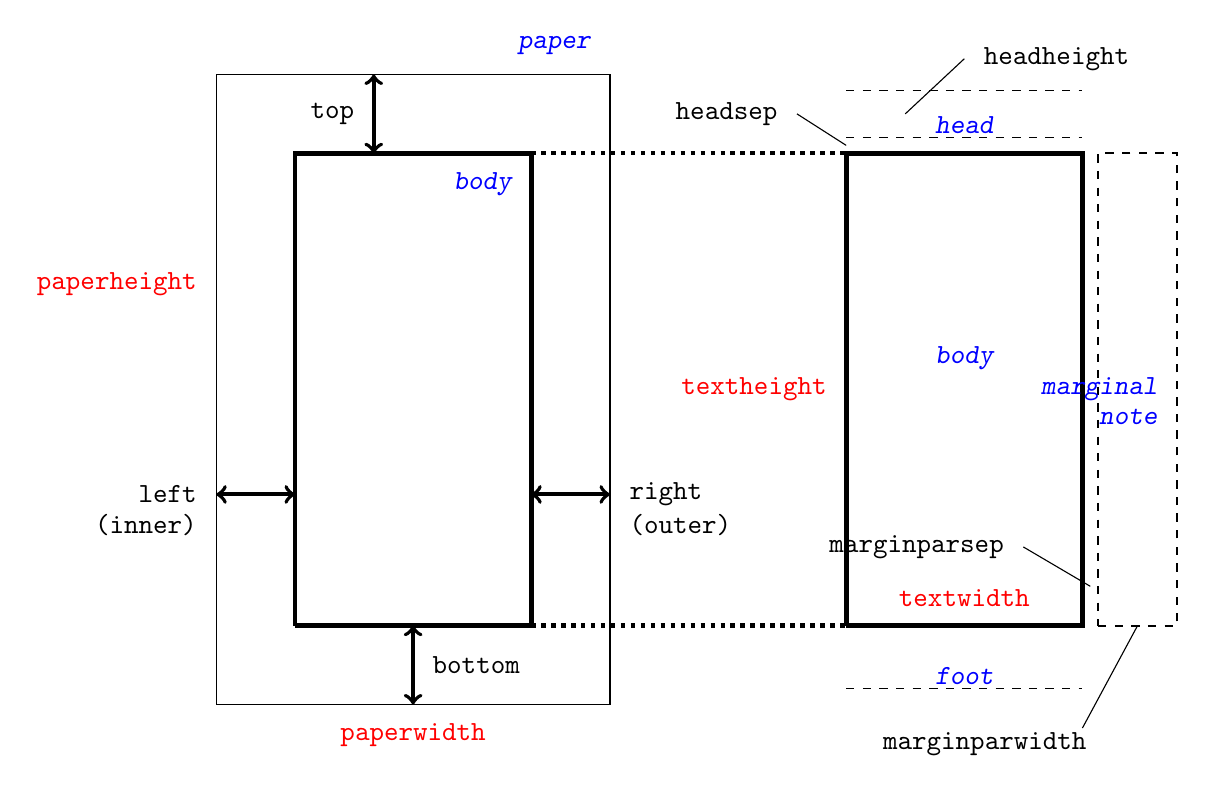
\begin{tikzpicture}{scale=0.9}
% outer-width & outer-height
\newcommand{\owd}{5};
\newcommand{\oht}{8};
% inner-width & inner-height
\newcommand{\iwd}{3};
\newcommand{\iht}{6};
% line length
\newcommand{\len}{5}

% Total Layout
\draw (0,0)--(\owd,0)--(\owd,\oht)--(0,\oht)--(0,0);
\draw[line width=0.06cm] (1,1)--(1+\iwd,1)--(1+\iwd,1+\iht)--(1,1+\iht)--(1,1);
\draw[ultra thick,dotted] (1+\iwd,1+\iht)--(\iwd+\len,1+\iht);
\draw[ultra thick,dotted] (1+\iwd,1)--(\iwd+\len,1);
% Arrow
\draw[<->,line width=0.05cm] (0,1/3*\oht)--(1,1/3*\oht);
\node[label=180:\texttt{left}] at (0,1/3*\oht){};
\node[label=225:\texttt{(inner)}] at (0,1/3*\oht){};
\draw[<->,line width=0.05cm] (1+\iwd,1/3*\oht)--(2+\iwd,1/3*\oht);
\node[label=0:\texttt{right}] at (2+\iwd,1/3*\oht){};
\node[label=315:\texttt{(outer)}] at (2+\iwd,1/3*\oht){};
\draw[<->,line width=0.05cm] (1+\iwd/2,1)--(1+\iwd/2,0);
\node[label=0:\texttt{bottom}] at (1+\iwd/2,0.5){};
\draw[<->,line width=0.05cm] (1+\iwd/3,1+\iht)--(1+\iwd/3,\oht);
\node[label=180:\texttt{top}] at (1+\iwd/3,1/2+\iht/2+\oht/2){};
% Outer Page Label
\node[label=135:\color{blue}{\ttfamily\slshape{paper}}] at (\owd,\oht){};
\node[label=225:\color{blue}{\ttfamily\slshape{body}}] at (1+\iwd,1+\iht){};

% Inner Page
\newcommand{\inn}{\iwd+\len};
\draw[line width=0.06cm] (\inn,1)--(\inn+\iwd,1)--(\inn+\iwd,1+\iht)--(\inn,1+\iht)--(\inn,1);
\node[label=180:\color{red}{\ttfamily{textheight}}] at (\inn,1+\iht/2){};
\node[label=90:\color{red}{\ttfamily{textwidth}}] at (\inn+\iwd/2,1){};
% Margin
\newcommand{\marsep}{0.2}
\newcommand{\marwd}{1}
\newcommand{\mar}{\inn+\iwd+\marsep}
\draw[thick,dashed] (\mar,1)--(\mar+\marwd,1)--(\mar+\marwd,1+\iht)--(\mar,1+\iht)--(\mar,1);
\draw (\mar-\marsep/2,1.5)--(\inn+3/4*\iwd,2);
\node[label=180:\texttt{marginparsep}] at (\inn+3/4*\iwd,2){};
\draw (\mar+\marwd/2,1)--(\inn+\iwd,-0.3);
\node[label=180:\texttt{marginparwidth}] at (\mar+\marsep/2,-0.5){};
% Foot
\draw[dashed] (\inn,0.2)--(\inn+\iwd,0.2);
\node[label=90:\color{blue}{\ttfamily\slshape{foot}}] at (\inn+\iwd/2,0){};
% Head
\draw[dashed] (\inn,1+\iht+0.8)--(\inn+\iwd,1+\iht+0.8);
\draw[dashed] (\inn,1+\iht+0.2)--(\inn+\iwd,1+\iht+0.2);
\node[label=90:\color{blue}{\ttfamily\slshape{head}}] at (\inn+\iwd/2,1+\iht){};
\draw (\inn,1+\iht+0.1)--(\inn-\len/8,1+\iht+0.5);
\node[label=180:\texttt{headsep}] at (\inn-\len/8,1+\iht+0.5){};
\draw (\inn+\iwd/4,1+\iht+0.5)--(\inn+\iwd/2,1+\iht+1.2);
\node[label=0:\texttt{headheight}] at (\inn+\iwd/2,1+\iht+1.2){};

% Total
\node[label=180:\color{red}{\ttfamily{paperheight}}] at (0,2/3*\oht){};
\node[label=270:\color{red}{\ttfamily{paperwidth}}] at (\owd/2,0){};
\node[label=\color{blue}{\ttfamily\slshape{body}}] at (\inn+\iwd/2,1+\iht/2){};
\node[label=180:\color{blue}{\ttfamily\slshape{marginal}}] at (\mar+\marwd,1+\iht/2){};
\node[label=225:\color{blue}{\ttfamily\slshape{note}}] at (\mar+\marwd,1+\iht/2){};
\end{tikzpicture}
\figcaption{页面构成示意图}
\label{fig:geo-paper}
\end{figure}

geometry宏包的具体的选项参数有:
\begin{feai}
\item \texttt{paper=<papername>:} 其中纸张尺寸有[a0--a6, b0--b6, c0--c6]paper, ansi[a--e]paper, letterpaper, executivepaper, legalpaper. 
\item \texttt{papersize=\{<width>,<height>\}}: 自定义尺寸。也可以单独对paperwidth或者paperheigth赋值。
\item \texttt{landscape}: 切换到横向纸张。默认的是portrait. 
\end{feai}

body部分分为两个概念:一个是总文本区(total body),另一个是主文本区(body). 总文本区可以由主文本区加上页眉(head)、页脚(foot)、侧页边(marginalpar)组成。默认的选项为includehead,表示总文本区包含页眉。要包括其他内容,可使用:\texttt{includefoot, includeheadfoot, includemp, includeall},以及以上各个参数将include改为ignore后的参数。

总文本区在默认状态下占纸张总尺寸的0.7,由scale=0.7控制,你也可以分别用\texttt{hscale}和\texttt{vscale}指定宽和高的占比。用具体的长度定义也是可以的,使用\texttt{(total)width}和\texttt{(total)height}定义总文本区尺寸,或者用\texttt{textwidth}和\texttt{textheight}定义主文本区的尺寸\footnote{当totalwidth和textwidth都定义时,优先采用后者的值。}。或者直接用\texttt{total=\{width,height\}, body=\{width,height\}}定义。甚至你可以用\texttt{lines=<num>}行数指定textheight。

页边的控制最为常用,分别用\texttt{left/inner, right/outer, top, bottom}来定义四向的页边。其中\texttt{inner, outer}参数只在文档的twoside参数启用时才有意义。你可以用\texttt{hmarginratio}来给定left(inner)与right(outer)页边宽的比例,默认是单页1:1、双页2:3。top和bottom之间的比由\texttt{vmarginratio}给定。你也可以用\texttt{vcentering, hcentering, centering}来指定页边比例为1:1. 在文档的左侧(内侧),可以指定装订线宽度\texttt{bindingoffset},使页边不会侵入。

页眉和页脚是位于top和bottom页边之内的文档元素。对于页眉和页脚的高度,分别使用\texttt{headheight/head, footskip/foot}参数指定。\texttt{marginpar}用来指定侧页边的宽度。它们到主文本区的参数分别是\texttt{headsep, footnotesep, marginparsep}. 你可以用\texttt{nohead, nofoot, nomarginpar}参数来清楚总文本区中的页眉,页脚和侧页边。

对于在文档类documentclass命令中能使用的参数,geometry有不少也能做。比如\texttt{twoside, onecolumn, twocolumn}。甚至还能用文档类中不能用的\texttt{columnsep}(启用多栏分隔线)。

最后,这是一个小例子:
\begin{latex}{}
\usepackage[marginpar=3cm, includemp]{package}
\end{latex}

\subsection{页眉和页脚}
主要借助fancyhdr宏包。\LaTeX 中的页眉页脚定义主要借助了两个命令,一个是\latexline{\\pagestyle},参数有:
\begin{para}
\item[empty] 无页眉页脚。
\item[plain] 无页眉,页脚只包含一个居中的页码。
\item[headings] 无页眉,页脚包含章/节名称与页码。
\item[myheadings] 无页眉,页脚包含页码和用户定义的信息。
\end{para}

另一个命令是\latexline{\\pagenumbering},与计数器一样,拥有\texttt{arabic, [Rr]oman, [Aa]lph}五种页码形式。

fancyhdr宏包给出了一个叫fancy的pagestyle,将页眉和页脚分别分为左中右三个部分,分别叫lhead, chead, rhead, 以及类似的[lcr]foot. 页眉页脚处的横线粗细也可以定义,默认页眉为0.4pt、页脚为0pt. 下面是一个例子:
\begin{latex}{}
\usepackage{fancyhdr}
\pagestyle{fancy}
  \lhead{}
  \chead{}
  \rhead{\bfseries wklchris}
  \lfoot{Leftfoot}
  \cfoot{\thepage}
  \rfoot{Rightfoot}
\renewcommand{\headrulewidth}{0.4pt}
\renewcommand{\footrulewidth}{0.4pt}
\end{latex}

加载这个宏包更多地是为了解决双页文档的排版问题。对于双页文档,fancyhdr宏包给出了一套新的指令:用E, O表示单数页和双数页,L, C, R表示左中右,H, F表示页眉和页脚。其中H, F需要配合\latexline{\\fancyhf}命令使用,比如\latexline{\\fancyhf[HC,FC]{This}}。如果不使用H, F参数,可以使用fancyhead, fancyfoot两个命令代替。一个新的例子:
\begin{latex}{}
\fancyhead{} % 清空页眉
  \fancyhead[RO,LE]{\bfseries wklchris}
\fancyfoot{} % 清空页脚
  \fancyfoot[LE,RO]{Leftfoot}
  \fancyfoot[C]{\thepage}
  \fancyfoot[RE,LO]{Rightfoot}
\end{latex}

fancyhdr在定义双页文档时,采用了如下的默认设置:
\begin{latex}{}
\fancyhead[LE,RO]{\slshape \rightmark}
\fancyhead[LO,RE]{\slshape \leftmark}
\fancyfoot[C]{\thepage}
\end{latex}

上例中的\latexline{\\rightmark}表示较低级别的信息,即当前页所在的section,形式如“1.2 sectionname ”,对于article则是subsection;而\latexline{\\leftmark}表示较高级别的信息,即对应的chapter,对于article则是section. 命令\latexline{\\leftmark}包含了页面上\latexline{\\markboth}\footnote{\latexline{\\markboth}是一个会被\latexline{\\chapter}等命令调用的命令,默认右参数是空。注意,带星号的大纲不调用这一命令,你需要这样书写:\latexline{\\chapter*{This\\markboth{This}{}}}。}下的最后一条命令的左参数,比如该页上出现了section 1--2,那么leftmark就是“Section 2”;命令\latexline{\\rightmark}则包含了页面上的第一个\latexline{\\markboth}命令的右参数或者第一个\latexline{\\markright}命令的唯一参数,比如可能是“Subsection 1.2”。

这听起来可能难以理解,但是markboth命令有两个参数,故有左右之分;而markright命令只有一个参数。你可以试着再去理解一下双页文档下的fancyhdr的默认设置。利用这一点来重定义chaptermark, sectionmark, subsectionmark(仅其中两项)命令,举个例子:
\begin{latex}{}
% 这里的参数#1是指输入的section/chapter的标题
% 效果:“1.2. The section”
\renewcommand{\sectionmark}[1]{\markright{\thesection.\ #1}}
% 效果:“CHAPTER 2. The chapter” 
\renewcommand{\chaptermark}[1]{\markboth{\MakeUppercase{%
  \chaptername}\ \thechapter.\ #1}{}}
\end{latex}

如果你对于默认的pagestyle不满意,可以用\latexline{\\fancypagestyle}命令进行更改。例如更改plain页面类型:
\begin{latex}{}
\fancypagestyle{plain}{
  \fancyhf{} % 清空页眉页脚
  \fancyhead[c]{\thesection}
  \fancyfoot{\thepage}}
\end{latex}

\section{抄录与代码环境}
抄录是指将键盘输入的字符(包括保留字符和空格)不经过\TeX 解释,直接输出到文档。默认的字体参数是等宽字族(ttfamily)。使用方法是\verb|\verb|命令或者verbatim(*)环境,区别在于带星号的环境会将空格以“\textvisiblespace”(\latexline{\\textvisiblespace})的形式标记出来。

注意,\verb|\verb|命令是一个特殊的命令,可以用一组花括号括住抄录内容,也可以任意两个同样的符号。比如:
\begin{latex}{}
\verb|fooo{}bar|
\verb+fooo{}bar+
\end{latex}

代码环境的输出,比如本文中带行号的代码块,参见\hyperref[sec:coding]{这一节}。

\section{分栏}
这部分内容使用\latexline{\\documentclass[twocolumn]{...}}这个可选参数就可以实现。如果在同一页内需要分栏与单栏并存(比如摘要跨栏,正文分栏),或者想要分三栏,请参考multicol宏包。

\section{文档拆分}
\label{sec:include}
文档拆分很简单,只需要把多个tex文件放在一起,然后再主文件中使用\latexline{\\input{filename}}或者\latexline{\\include{filename}}命令就可以了,带不带扩展名均可。两个命令区别在于\latexline{\\include}命令将会很好地支持大纲编号。

拆分的优势在于可以根据chapter(或其他)分为多个文件,省去了长文档浏览时的一些不便。你也可以把整个导言区做成一个文件,然后在不同的\LaTeX 文档中反复使用,即充当模板的功能。你还可以把较长的tikz绘图代码写到一个tex中,在需要时\latexline{\\input}即可。

\section{西文排版及其他}
\subsection{连写}
\LaTeX 排版以及正规排版中,如果你输入ff, fl, fi, ffi等内容,它们默认会连写。在字母中间插入空白的箱子以强制不连写:\latexline{f\\mbox{}l}。

\subsection{断词}
行末的英文单词太长,\LaTeX 就会以其音节断词。如果你想指定某些单词的断词位置,使用如下命令断词。例子:
\begin{latex}{}
\hyphenation{Hy-phen-a-tion FORTRAN}
\end{latex}

这个例子允许Hyphenation, hyphenation在短横处断词,同时\textbf{禁止}FORTRAN, Fortran, fortran断词。如果你在行文中加入\verb|\-|命令,则可以实现允许在对应位置断词的效果。比如:

\begin{codeshow}
I will show you this example:
su\-per\-cal\-i\-frag\-i\-lis\-%
tic\-ex\-pi\-al\-i\-do\-cious
\end{codeshow}

如果你不想断词,比如电话号码,巧妙利用\latexline{\\mbox}命令吧:
\begin{latex}{}
My telephone number is: \mbox{012 3456 7890}
\end{latex}

\subsection{特殊符号}
符号的总表可以参照symbols-a4文档,运行texdoc symbols-a4即可调出。包括希腊字母在内的一些数学符号将会在下一章介绍。这里给出基于wasysym宏包的一些常用符号:
\begin{center}
  \centering
  \tabcaption{wasysym宏包符号}
  \begin{tabular}{*{3}{c >{\ttfamily\char92}p{5em}}}
     \permil     & permil   & \male     & male  & \female       & female \\
     \checked    & checked  & \XBox     & XBox  & \CheckedBox   & CheckedBox \\
     \hexstar    & hexstar  & \phone    & phone & \twonotes     & twonotes
  \end{tabular}
\end{center}

\subsection{其他}
如果你想在某个不带参数的命令后输入空格,请接上一个空的花括号确保空格能够正常输出。例如:\latexline{这是\\TeX{} Live. }

\chapter{数学排版}
\section{行间与行内公式}
\co{行内公式}指将公式嵌入到文段的排版方式,主要要求公式垂直距离不能过高,否则影响排版效果。行内公式的书写方式:
\begin{latex}{}
$...$ 或者 \(...\) 或者 \begin{math}...\end{math}
\end{latex}

一般推荐第一种方式。例如:\verb|$\sum_{i=1}^{n}a_i$|,即:$\sum_{i=1}^{n}a_i$. 

另外一种公式排版方式是\co{行间公式},也称行外公式,使用:
\begin{latex}{}
\[...\] 或者 \begin{displaymath}...\end{displaymath}
或者 amsmath 提供的\begin{equation*}...\end{equation*}
\end{latex}

一般也推荐第一种命令\footnote{还有一种\texttt{\$\$...\$\$}的写法,问题很多,绝不建议使用。},例如:\verb|\[\sum_{i=1}^n{a_i}\]|,得到:

\[\sum_{i=1}^{n}a_i\]

从上面的两个例子可以看出,即使输出相同的内容,行内和行间的排版也是有区别的,比如累计符号上标是写在正上方还是写在右上角。

如果行间公式需要编号,使用equation环境\footnote{需要注意有一个\RED{已经淘汰}的多行公式编号环境叫\texttt{eqnarray},请不要再使用。},还可以插入标签:

\begin{codeshow}
\begin{equation}
\label{eq:NoExample}
  |\epsilon|>M
\end{equation}
\end{codeshow}

\section{数学字体、字号与空格}
\label{sec:mathfont}
\subsection{空格}
在数学环境中,行文空格是被忽略的。比如\verb|$x,y$|和\verb|$x, y$|并没有区别。数学环境有独有的空格命令:

\begin{codeshow}
  $没有空格,3/18空\,格$ \\
  $4/18空\:格,5/18空\;格$ \\
  $9/18空\ 格,一个空\quad 格$ \\
  $两个空\qquad 格,负3/18空\!格$
\end{codeshow}

事实上,以上命令也可以在数学模式外使用,其中使用最广泛的是\verb|\,|,比如上文提到过的千位分隔符。在数学环境中它也应用广泛:

\begin{codeshow}
\[ \int_0^1 x \ud{}x
= \frac{1}{2} \]
\end{codeshow}

其中\verb|\ud|命令是自定义的,这也是微分算子的正常定义\label{cmd:ud}:
\begin{latex}{}
\newcommand{\ud}{\mathop{}\negthinspace\mathrm{d}}
\end{latex}

\subsection{数学字体}
将字体转为正体使用\latexline{\\mathrm}命令。如果需要保留行文中的空格,使用\latexline{\\textrm}命令——这个与正文一致。但是,textrm命令内的字号可能不会自适应,mathrm则稳定得多。

例如自然对数的底数$\ue$,在本文中就是这样定义的:
\begin{latex}{}
\newcommand{\ue}{\mathrm{e}}
\end{latex}

以下简单介绍几种数学字体。数学字体的总表参见\tref{tab:mathfont}。

\subsubsection{数学粗体}
数学粗体使用amsmath宏包支持的\latexline{\\boldsymbol}命令。命令\latexline{\\boldmath}的问题在于它只能加粗一个数学环境,其中很可能包括了标点符号,而这时不严谨的。命令\latexline{\\mathbf}就差的更远,它只能把字体转为\textbf{正}粗体,而数学字体都是斜体的。

\begin{codeshow}
$\mu,M$\\
$\boldsymbol{\mu},
\boldsymbol{M}$ \\
\end{codeshow}

\subsubsection{空心粗体}
空心粗体使用amsfonts或者amssymb宏包的\latexline{\\mathbb}命令。这里使用\latexline{\\textrm}而不是\latexline{\\mathrm},是为了保留空格。

\begin{codeshow}
$x^2 \geq 0 \qquad
\textrm{for all }x\in\mathbb{R}$
\end{codeshow}

\section{基本命令}
基本函数默认用正体书写,包括:
\begin{verbatim}
\sin \cos \tan \arcsin \arccos \arctan \cot \sec \csc
\sinh \cosh \tanh \coth \log \lg \ln \det
\exp \max \min \lim \dim \inf \liminf \sup \limsup
\deg \arg \hom \ker \gcd \Pr
\end{verbatim}

此外有一个叫\latexline{\\mathop}的命令,可以把任何的数学字符串转换为数学对象,使其适用上标、下标等数学对象才能使用的命令。

\subsection{上下标与虚位}
用低划线和尖角符表示上标和下标,请仔细体会下述例子:

\begin{codeshow}
$a^3_{ij}$ \\
${a_{ij}}^3\text{或}a_{ij}{}^3$\\
$\mathrm{e}^{x^2}\geq 1$
\end{codeshow}

上面的指数3的位置读者可以多多体会一下。此外,\verb|\phantom|被称为虚位命令,从下例你也能够体会到他的作用:

\begin{codeshow}
${}^{12}_{6}\mathrm{C}$ \\
${}^{12}_{\phantom{1}6}
\mathrm{C}$ \\
$a^3_{ij}$ \\
$a^{\phantom{ij}3}_{ij}$
\end{codeshow}

\subsection{微分与积分}
导数直接使用单引号\verb|'|,积分使用\verb|\int|符号:

\begin{codeshow}
$y'=x \qquad \dot{y}(t)=t$ \\
$\ddot{y}(t)=t+1$
$\dddot{y}+\ddddot{y}=0$ \\
$\iint_{D}f(x)=0$
$\int_{0}^{1}f(x)=1$
\end{codeshow}

有时候需要更高级的微分或积分号,其中\latexline{\\ud}命令在\hyperref[cmd:ud]{上文这里}定义过:
\begin{latex}{}
\[\left.\frac{\ud y}{\ud x}\right|_{x=0}
\quad\frac{\partial f}{\partial x}
\quad\oint\;\varoiint_S \]
\end{latex}

效果:
\[\left.\frac{y}{x}\right|_{x=0}
\quad\frac{\partial f}{\partial x}\quad
\oint\;\varoiint_S \]

其中的\verb|\dot|系的导数形式\LaTeX 只原生支持到二阶导数。后面的三阶、四阶需要amsmath宏包。\verb|\int|系的积分命令也是一样。而环形双重积分命令\verb|\varoiint|需要esint宏包\footnote{该宏包可能与amsmath冲突,即便使用也请其放在amsmath之后加载。}。

\verb|\left.|或\verb|\right.|命令\footnote{参考\hyperref[subsec:delimiter]{定界符}部分的内容。}只用于匹配,本身不输出任何内容。

\subsection{分式、根式与堆叠}
分式使用\verb|\frac|命令。或者amsmath宏包支持的\latexline{\\dfrac}命令来强制获得行间公式大小的分数,\latexline{\\tfrac}则强制获得行内公式大小的分数:

\begin{codeshow}
  $\sqrt{\frac{x}{y}}$ \\
  $x^{1/2} \qquad x^{1\frac{2}{3}}$
\end{codeshow}

根式:

\begin{codeshow}
  $\sqrt{2} \quad \surd$ \\
  $\sqrt[3]{\sqrt{2}+1}$
\end{codeshow}

划线命令使用\verb|\underline|和\verb|\overline|,水平括号使用brace:

\begin{codeshow}
$\overline{m+n}$ \\
$\underbrace{a_1+\ldots+a_n}_{n}$
$\overbrace{a_1+\ldots+a_n}^{n}$
\end{codeshow}

事实上\verb|\overline|命令也存在问题,请比较:

\begin{codeshow}
$\overline{A}\overline{B}$ \\
$\closure{A}\closure{B}$
$\closure{AB}$
\end{codeshow}

其中closure是在导言区定义的
\begin{latex}{}
\newcommand{\closure}[2][3]{{}\mkern#1mu\overline{\mkern-#1mu#2}}
\end{latex}

向量符号:

\begin{codeshow}
  $\vec a\quad\overrightarrow{PQ}$
  $\overleftarrow{EF}$
\end{codeshow}

尖帽符号或者波浪符号:

\begin{codeshow}
  $\hat{A} \quad \widehat{AB}$ \\
  $\tilde{C} \quad \widetilde{CD}$
\end{codeshow}

强制堆叠命\latexline{\\stackrel},位于上方的符号与上标同等大小。如果有amsmath宏包,可以使用\latexline{\\overset}或者\latexline{\\underset} 命令,前者与\latexline{\\stackrel}命令完全等同:

\begin{codeshow}
  $\int f(x) \stackrel{?}{=} 1$\\
  $A\overset{abc}{=}B$ \quad
  $C\underset{def}{=}D$
\end{codeshow}

还有一个很强大的堆叠放置命令\verb|\sideset|:

\begin{codeshow}
\[\sideset{_a^b}{_c^d}\sum\]
\[\sideset{}{'}\sum_{n=1}\text{或}
\,{\sum\limits_{n=1}}'\]
\end{codeshow}

去心邻域大概也属于堆叠符的一种?这样输出:

\begin{codeshow}
$\mathring{U}$
\end{codeshow}

在下一次节:累加与累积中,还介绍了更多的堆叠命令。

\subsection{累加与累积}
使用\verb|\sum|和\verb|\prod|命令,效果如下:

\begin{codeshow}
\[\sum_{i=1}^{n}a_i=1 \qquad
\prod_{j=1}^{n}b_j=1\]
\end{codeshow}

有时需要复杂的堆叠方式,效果如下:

\begin{codeshow}
\[\sum_{\substack{0<i<n \\
  0<j<m}} p_{ij}=
  \prod_{\begin{subarray}{l}
  i\in I \\  1<j<m
  \end{subarray}}q_{ij}\]
\end{codeshow}

有时候需要强制实现堆叠的效果,可以使用\latexline{\\limits}命令。如果堆积目标不是数学对象,还需要使用\latexline{\\mathop}命令:

\begin{codeshow}
\[\max\limits_{i>1}^{x}\quad
\mathop{xyz}\limits_{x>0}\quad
\lim\nolimits_{x\to \infty}\]
\end{codeshow}

\subsection{矩阵与省略号}
矩阵的排版可以通过array环境和自适应定界符完成:

\begin{codeshow}
\[\mathbf{A}=
\left(\begin{array}{ccc}
x_{11} & x_{12} & \ldots \\
x_{21} & x_{22} & \ldots \\
\vdots & \vdots & \ddots
\end{array}\right)\]
\end{codeshow}

还有就是\verb|\cdots|命令。hmath宏包还提供了一种省略号\verb|\adots|:$\adots$,或许用得上呢?

\LaTeX 原生支持自动添加定界符的形式,不过要放在数学环境内:

\begin{codeshow}
\centering $\begin{matrix}
0 & 1 \\ 1 & 0 \end{matrix}\qquad
\begin{pmatrix} 0 & 2 \\
2 & 0 \end{pmatrix}$
\end{codeshow}

方括号和花括号使用\verb|\bmatrix|命令:

\begin{codeshow}
\centering $\begin{bmatrix}
0 & 3 \\ 3 & 0 \end{bmatrix}\qquad
\begin{Bmatrix} 0 & 4 \\
4 & 0 \end{Bmatrix}$
\end{codeshow}

行列式使用\verb|\vmatrix|命令:

\begin{codeshow}
\centering $\begin{vmatrix}
0 & 5 \\ 5 & 0 \end{vmatrix}\qquad
\begin{Vmatrix} 0 & 6 \\
6 & 0 \end{Vmatrix}$
\end{codeshow}

array环境还有更多的用途,也可以像表格一样划线:

\begin{codeshow}
\[\begin{array}{c|c}
  a_{11} & a_{12} \\
  \hline
  a_{21} & a_{22}
  \end{array}\]
\end{codeshow}

\subsection{分段函数与联立方程}
array也可以用来写分段函数:

\begin{codeshow}
\[y=\left\{\begin{array}{ll}
x+1, & x>0 \\
0,   & x=0 \\
x-1, & x<0
\end{array}\right.\]
\end{codeshow}

分段函数还能用cases环境,它自动生成一个花括号,也更紧凑:

\begin{codeshow}
\[y=\begin{cases}
\int x, & x>0 \\
0,   & x=0 \\
x-1, & x<0
\end{cases},\,
x\in\mathbb{R}\]
\end{codeshow}

如果想要生成display样式的内容(比如上面的积分号只是text样式的),使用mathtools宏包的dcases环境代替cases环境。如果cases环境的第二列条件不是数学语言而是一般文字,可以考虑使用dcases*环境,列中用\&{}隔开。

\begin{codeshow}
\[y=\begin{dcases}
  \int x, & x>0 \\
  x^2, & x\leqslant 0
  \end{dcases}\]
\[z=\begin{dcases*}
  y, & when $y$ is prime\\
  y^2, & otherwise
  \end{dcases*}\]
\end{codeshow}

\subsection{多行公式及其编号}
多行公式可以使用amsmath下的align环境——因为原生的eqnarray环境真的很差!而且align环境不需要像array环境那样给出列的数目和参数,能够根据
\texttt{\&}符号的数量来自调整。\qd{这个环境会自动对齐等号或者不等号,所以必要时请用\&指定对齐位置}。下面是一个例子:

\begin{codeshow}
\begin{align}
  a^2  &= a\cdot a \\
       &= a*a      \\
       &= a^2
\end{align}
\end{codeshow}

\LaTeX 中长公式不能自动换行\footnote{不过breqn宏包的dmath环境可以实现自动换行,读者可以自行尝试。},请自行指定断行位置和缩进距离,就像上面一样。也许你不需要三个编号,你可以:

\begin{codeshow}
\begin{align}
  a^2&= a\cdot a& b&=c\nonumber\\
  g  &= a*a & d&>e>f  \nonumber\\
  step&= a^2 & &Z^3
\end{align}
\end{codeshow}

如果你想让编号显示在这三行的中间而不是最下面一行,可以尝试把公式写在array环境中,然后再嵌套到equation环境内。如果你根本不想给多行公式编号,尝试align*环境。

如果想在环境中插入小段行间文字,使用intertext命令,或者mathtools宏包的shortintertext命令。区别是后者的垂直间距更小一些。

\begin{codeshow}
\begin{align*}
\shortintertext{If}
 y &= 0 \\
 x &< 0\\
\shortintertext{then}
 z &= x+y
\end{align*}
\end{codeshow}

当然,align环境是用来分列对齐的。如果你仅仅想要所有行居中,使用amsmath宏包的gather环境即可。这是一个非常实用的环境,你也可以用gather*环境排版居中的、非编号的多行公式。

\begin{codeshow}
\begin{gather}
  X=1+2+\cdots+n \\
  Y=1
\end{gather}
\end{codeshow}

\subsection{二项式与定理}
二项式可能需要借助amsmath宏包的\verb|\binom|命令:

\begin{codeshow}
  $\mathrm{C}_n^k=\binom{n}{k}$
\end{codeshow}

\RED{在使用这部分内容时,请加载amsthm宏包}。

首先是定理环境格式的自定义。如同定义命令一样,在导言区加上:

\noindent\begin{tabular}{|l|}
\hline
\char92{}newtheorem\{\textit{name}\}[\textit{counter}]\{\textit{text}\}[\textit{section}] \\
\hline
\end{tabular}

其中\textit{name}表示定理的引用名称,即下文将其作为一个环境名来识别;\textit{text}表示定理的显示名称,即下文中定理将以其作为打印内容。而\textit{counter}参数表示你是否与先前声明的某定理共同编号。\textit{section}参数表示定理的计数层级,如果是section,表示每节分别计数;chapter表示每章分别计数。

来看一个例子。首先在导言区定义如下三个样式:
\begin{verbatim}
\theoremstyle{definition}\newtheorem{laws}{Law}[section]
\theoremstyle{plain}\newtheorem{ju}[laws]{Jury}
\theoremstyle{remark}\newtheorem*{marg}{Margaret}
\end{verbatim}

以上三个theoremstyle即是它预定义的所有样式类型。definition标题粗体,内容罗马体;plain标题粗体,内容斜体;remark标题斜体,内容罗马体。带星号表示不进行计数。在环境的使用中可以添加可选参数,用于以括号的形式注释定理。然后这是示例:

\begin{codeshow}
\begin{laws}
Never believe easily.
\end{laws}
\begin{ju}[The 2nd]
Never suspect too much.
\end{ju}
\begin{marg}Nothing else.\end{marg}
\end{codeshow}

amsthm宏包也提供了proof环境,并且用\latexline{\\qedhere}来指定证毕符号的位置。如果不加指定,将会自动另起一行。

\begin{codeshow}
\begin{proof}
For an right triangle, we have:
  \[a^2+b^2=c^2 \qedhere\]
\end{proof}
\end{codeshow}

\section{数学符号与字体}
\subsection{数学字体}
原生的数学字体命令:
\begin{center}
\tabcaption{原生数学字体表}
\label{tab:mathfont}
\begin{tabular}{>{\ttfamily\char92}l>{$}l<{$}}
\hline
mathrm\{ABCDabcde 1234\} & \mathrm{ABCDabcde 1234} \\
\hline
mathit\{ABCDabcde 1234\} & \mathit{ABCDabcde 123} \\
\hline
mathnormal\{ABCDabcde 1234\} & \mathnormal{ABCDabcde 1234} \\
\hline
mathcal\{ABCDabcde 1234\} & \mathcal{ABCDabcde 1234} \\
\hline
\end{tabular}
\end{center}

需要其他宏包支持的数学字体:
\begin{center}
\tabcaption{宏包数学字体表}
\label{tab:mathfont-pk}
\begin{tabular}{>{\ttfamily\char92}ll}
\hline
mathscr\{ABCDabcde 1234\} & mathrsfs\\
$\mathscr\{ABCDabcde 1234\}$ & \\
\hline
mathfrak\{ABCDabcde 1234\} & amsfonts或者amssymb\\
$\mathfrak\{ABCDabcde 1234\}$ & \\
\hline
mathbb\{ABCDabcde 1234\} & amsfonts或者amssymb\\
$\mathbb\{ABCDabcde 1234\}$ & \\
\hline
\end{tabular}
\end{center}

\subsection{定界符}
\label{subsec:delimiter}
\tref{tab:delimiter}给出了一些数学环境中使用的定界符。

\begin{table}[!htb]
\centering
\caption{定界符}
\label{tab:delimiter}
\begin{tabular}{@{}*{3}{>{$}p{2em}<{$} @{} >{\ttfamily}p{7em}}}
( & ( & [ & [ or \char92 lbrack & \uparrow & \char92 uparrow \\
) & ) & ] & ] or \char92 rbrack & \downarrow & \char92 downarrow \\
\{ & \{ or \char92 lbrace & \} & \} or \char92 rbrace & \updownarrow & \char92 updownarrow \\
\langle & \char92 langle & \rangle & \char92 rangle & \backslash & \char92 backslash \\
\lfloor & \char92 lfloor & \rfloor & \char92 rfloor & \Updownarrow & \char92 Updownarrow \\
\lceil & \char92 lceil & \rceil & \char92 rceil & \Uparrow & \char92 Uparrow \\
\Vert & \char92 | or \char92 Vert & | & | or \char92 vert & \Downarrow & \char92 Downarrow \\
\hline
\multicolumn{6}{c}{-- 以下需要amssymb宏包 --} \\
\multicolumn{3}{c}{$\ulcorner$ \quad \texttt{\char92 ulcorner}} & \multicolumn{3}{c}{$\urcorner$ \quad \texttt{\char92 urcorner}} \\
\multicolumn{3}{c}{$\llcorner$ \quad \texttt{\char92 llcorner}} & \multicolumn{3}{c}{$\lrcorner$ \quad \texttt{\char92 lrcorner}}
\end{tabular}
\end{table}

使用\verb|\left|或者\verb|\right|能够使定界符自适应式子的高度:

\begin{codeshow}
\[\left\{x+\frac{\left[\left|\frac
{y}{x}\right|^3-Z^{5\left(\frac{x}
{y}+z\right)}\right]}{y}\right\}\]
\end{codeshow}

有时\verb|\left.|和\verb|\right.|能灵活地用于跨行控制,因为它们并非实际配对:

\begin{codeshow}
\begin{align*}
  x &=\left(\frac{1}{2}x\right.\\
  &\left.\vphantom{\frac{1}{2}}
  +y^2+z_1\right)
\end{align*}
\end{codeshow}

其中\verb|\vphantom|命令用于输出一个高度虚位,使得第二行的自适应定界符与第一行同等大小。

有时你可能希望手动指定定界符的尺寸,这时使用:

\begin{codeshow}
  $(\big(\Big(\bigg(\Bigg($ \\
  \[\bigl[\frac{x+y}{x^2}\bigr]\]
\end{codeshow}

\subsection{希腊字母}
希腊字母表如\tref{tab:greekletter}所示。表中包含了小写希腊字母、大写希腊字母,其中部分希腊字母的输入方式与英文字母一致。
\begin{table}[!htb]
\centering
\caption{希腊字母表}
\label{tab:greekletter}
\begin{tabular}{*{4}{>{$}p{2em}<{$} @{} >{\ttfamily\char92}p{6em} @{}}}
\alpha & alpha & \theta & theta & o & \multicolumn{1}{p{6em}}{o} & \upsilon & upsilon \\
\beta & beta & \vartheta & vartheta & \pi & pi & \phi & phi \\
\gamma & gamma & \iota & iota & \varpi & varpi & \varphi & varphi \\
\delta & delta & \kappa & kappa & \rho & rho & \chi & chi \\
\epsilon & epsilon & \lambda & lambda & \varrho & varrho & \psi & psi \\
\varepsilon & varepsilon & \mu & mu & \sigma & sigma & \omega & omega \\
\zeta & zeta & \nu & nu & \varsigma & varsigma & \eta & eta \\
\xi & xi & \tau & tau & \multicolumn{4}{c}{} \\
A & \multicolumn{1}{p{6em}}{A} & B & \multicolumn{1}{p{6em}}{B} & \Gamma & Gamma & \varGamma & varGamma \\
\Delta & Delta & \varDelta & varDelta & E & \multicolumn{1}{p{6em}}{E} & Z & \multicolumn{1}{p{6em}}{Z} \\
H & \multicolumn{1}{p{6em}}{H} & \Theta & Theta & \varTheta & varTheta & I & \multicolumn{1}{p{6em}}{I} \\
\Lambda & Lambda & \varLambda & varLambda & M & \multicolumn{1}{p{6em}}{M} & N & \multicolumn{1}{p{6em}}{N} \\
\Xi & Xi & \varXi & varXi & O & \multicolumn{1}{p{6em}}{O} & \Pi & Pi \\
\varPi & varPi & P & \multicolumn{1}{p{6em}}{P} & \Sigma & Sigma & \varSigma & varSigma \\
T & \multicolumn{1}{p{6em}}{T} & \Upsilon & Upsilon & \varUpsilon & varUpsilon & \Phi & Phi \\
\varPhi & varPhi & X & \multicolumn{1}{p{6em}}{X} & \Psi & Psi & \varPsi & varPsi \\
\Omega & Omega & \varOmega & varOmega & \multicolumn{4}{c}{}
\end{tabular}
\end{table}

\subsection{二元运算符}
二元运算符包括常见的加减乘除,还有集合的交、并、补等运算。\tref{tab:operator}只列出常用的二元运算符,更多的请参考symbols-a4文档。
\begin{table}[!htb]
\centering
\caption{二元运算符}
\label{tab:operator}
\begin{tabular}{@{}*{4}{>{$}p{2em}<{$} @{} >{\ttfamily\char92}p{6em} @{}}}
+ & \multicolumn{1}{p{6em}}{+} & - & \multicolumn{1}{p{6em}}{-} & \times & times & \div & div \\
\pm & pm & \mp & mp & \circ & circ & \triangleright & triangleright \\
\cdot & cdot & \star & star & \ast & ast & \triangleleft & triangleleft \\
\cup & cup & \cap & cap & \setminus & setminus & \bullet & bullet \\
\oplus & oplus &\ominus & ominus & \otimes & otimes & \oslash & oslash \\
\odot & odot & \bigcirc & bigcirc & \vee & vee,lor & \wedge & wedge,land \\
\bigcup & bigcup & \bigcap & bigcap & \bigvee & bigvee & \bigwedge & bigwedge
\end{tabular}
\end{table}

\subsection{二元关系符}
二元关系符常常被用于判断两个数的大小关系,或者集合中的从属关系。\tref{tab:relation-operator}和\tref{tab:amsrelation-operator}只列出常用的二元关系符,更多的请参考symbols-a4文档。
\begin{table}[!htb]
\centering
\caption{二元关系符}
\label{tab:relation-operator}
\begin{tabular}{@{}*{4}{>{$}p{2em}<{$} @{} >{\ttfamily\char92}p{6em} @{}}}
< & \multicolumn{1}{p{6em}}{<} & > & \multicolumn{1}{p{6em}}{>} & \le & le(q) & \ge & ge(q) \\
\ll & ll & \gg & gg & \equiv & equiv & \neq & neq \\
\prec & prec & \succ & succ & \preceq & preceq & \succeq & succeq \\
\sim & sim & \simeq & simeq & \cong & cong & \approx & approx \\
\subset & subset & \supset & supset & \subseteq & subseteq & \supseteq & supseteq \\
\in & in & \ni & ni & \notin & notin & \propto & propto \\
\parallel & parallel & \perp & perp & \smile & smile & \frown & frown \\
\asymp & asymp & \bowtie & bowtie & \vdash & vdash & \dashv & dashv
\end{tabular}
\end{table}

\tref{tab:amsrelation-operator}中的二元关系符需要amssymb宏包。
\begin{table}[!htb]
\centering
\caption{amssymb二元关系符}
\label{tab:amsrelation-operator}
\begin{tabular}{@{}*{4}{>{$}p{2em}<{$} @{} >{\ttfamily\char92}p{6em} @{}}}
\leqslant & leqslant & \geqslant & geqslant & \because & because & \therefore & therefore \\
\nless & nless & \ngtr & ngtr & \lessdot & lessdot & \gtrdot & gtrdot \\
\lessgtr & lessgtr & \gtrless & gtrless & \lesseqqgtr & lesseqqgtr & \gtreqqless & gtreqqless \\
\subseteqq & subseteqq & \supseteqq & supseteqq & \subsetneqq & subsetneqq & \supsetneqq & supsetneqq
\end{tabular}
\end{table}

\subsection{箭头}
在\tref{tab:delimiter}中给出了几个箭头符号,但是不够全,这里给出总表如\tref{tab:arrow}。
\begin{table}[!htb]
\centering
\caption{箭头}
\label{tab:arrow}
\begin{tabular}{@{}*{2}{>{$}p{3em}<{$} @{} >{\ttfamily\char92}p{10em} @{}}}
\leftarrow & leftarrow & \longleftarrow & longleftarrow \\
\rightarrow & rightarrow & \longrightarrow & longrightarrow \\
\leftrightarrow & leftrightarrow & \longleftrightarrow & longleftrightarrow \\
\Leftarrow & Leftarrow & \Longleftarrow & Longleftarrow \\
\Rightarrow & Rightarrow & \Longrightarrow & Longrightarrow \\
\Leftrightarrow & Leftrightarrow & \Longleftrightarrow & Longleftrightarrow \\
\mapsto & mapsto & \longmapsto & longmapsto \\
\nearrow & nearrow & \searrow & searrow \\
\swarrow & swarrow & \nwarrow & nwarrow \\
\leftharpoonup & leftharpoonup & \rightharpoonup & rightharpoonup \\
\leftharpoondown & leftharpoondown & \rightharpoondown & rightharpoondown \\
\rightleftharpoons & rightleftharpoons & \iff & iff (bigger space)
\end{tabular}
\end{table}

依旧给出一个基于amssymb宏包的附\tref{amsarrow}。
\begin{table}[!htb]
\centering
\caption{amssymb箭头}
\label{tab:amsarrow}
\begin{tabular}{@{}*{2}{>{$}p{3em}<{$} @{} >{\ttfamily\char92}p{10em} @{}}}
\dashleftarrow & dashleftarrow & \dashrightarrow & dashrightarrow \\
\circlearrowleft & circlearrowleft & \circlearrowright & circlearrowright \\
\leftrightarrows & leftrightarrows & \rightleftarrows & leftrightarrows \\
\nleftarrow & nleftarrow & \nLeftarrow & nLeftarrow \\
\nrightarrow & nrightarrow & \nRightarrow & nRightarrow \\
\nleftrightarrow & nleftrightarrow & \nLeftrightarrow & nLeftrightarrow
\end{tabular}
\end{table}

\subsection{其他符号}
最后是一些其他的难以归类的符号,也不全是数学领域会用到的,只不过它们可以在数学环境下输出出来,以及被amssymb宏包所支持。如\tref{tab:othersym}和\tref{tab:amsothersym}。
\begin{table}[!htb]
\centering
\caption{其他符号}
\label{tab:othersym}
\begin{tabular}{@{}*{4}{>{$}p{2em}<{$} @{} >{\ttfamily\char92}p{5.5em} @{}}}
\dots & dots & \cdots &cdots &
\vdots & vdots & \ddots & ddots \\
\forall & forall & \exists & exists &
\Re & Re & \aleph & aleph \\
\angle & angle & \infty & infty &
\triangle & triangle & \nabla & nabla \\
\hbar & hbar & \imath & imath &
\jmath & jmath & \ell & ell \\
\spadesuit & spadesuit & \heartsuit & heartsuit &
\clubsuit & clubsuit & \diamondsuit & diamondsuit \\
\flat & flat & \natural & natural &
\sharp & sharp & & \\
\hline
\multicolumn{8}{l}{非数学符号:} \\
\multicolumn{1}{p{2em}}{\pounds} & pounds & \multicolumn{1}{p{2em}}{\S} & S &
\multicolumn{1}{p{2em}}{\copyright} & copyright & \multicolumn{1}{p{2em}}{\P} & P \\
\multicolumn{1}{p{2em}}{\dag} & dag & \multicolumn{1}{p{2em}}{\ddag} & ddag &
\multicolumn{1}{p{2em}}{\textregistered} & \multicolumn{3}{l}{textregistered}
\end{tabular}
\end{table}

\begin{table}[!htb]
\centering
\caption{amssymb其他符号}
\label{tab:amsothersym}
\begin{tabular}{@{} >{$}p{2em}<{$} @{} >{\ttfamily\char92}p{6em} @{}*{2}{>{$}p{2em}<{$} @{} >{\ttfamily\char92}p{9em} @{}}}
\square & square & \blacksquare & blacksquare & \hslash & hslash \\
\bigstar & bigstar & \blacktriangle & blacktriangle & \blacktriangledown & blacktriangledown \\
\lozenge & lozenge & \blacklozenge & blacklozenge & \measuredangle & measuredangle \\
\mho & mho & \varnothing & varnothing & \eth & eth
\end{tabular}
\end{table}

\clearpage
\chapter{\LaTeX{}进阶}
本章的内容多数与宏包的使用相关。记得使用texdoc命令查看宏包的使用手册,这是学习宏包最好的手段,没有之一。

\section{自定义命令与环境}
\label{sec:newcommand}
自定义命令是\LaTeX 相比于字处理软件MS Word之流最强大的功能之一。它可以大幅度优化你的文档体积,用法是:
\begin{latex}{}
\newcommand{cmd}[args][default]{def}
\end{latex}

现在来解释一下各个参数:
\begin{para}
\item[cmd:] 新定义的命令,不能与现有命令重名。
\item[args:] 参数个数。
\item[default:] 首个参数,即\texttt{\#{}1}的默认值。
\item[def:] 具体的定义内容。参数1以\texttt{\#{}1}代替,参数2以\texttt{\#{}2}代替,以此类推。
\end{para}

如果重定义一个现有命令,使用\latexline{\\renewcommand}命令,用法与\latexline{\\newcommand}一致。简单的例子:
\begin{latex}{}
% 加粗:\concept{text}
\newcommand{\concept}[1]{\textbf{#1}}
% 加粗#2并把#1#2加入索引,默认#1为空。
% 比如\cop{Sys}或者\cop[Sec.]{Sys}
\newcommand{\cop}[2][]{\textbf{#2}}\index{#1 #2}}
\end{latex}

\section{箱子:排版的基础}
\label{sec:box}
\LaTeX 排版的基础单位就是“箱子(box)”,例如整个页面是一个矩形的箱子,侧边栏、主正文区、页眉页脚也都是箱子。在正常排版中,文字应当位于箱子内部;如果单行文字过长、没能正确断行,造成文字超出箱子,这便是Overfull的坏箱(bad box);如果内容太少,导致文字不能美观地填满箱子,便是Underfull的坏箱。

在\LaTeX 编译中,坏箱将记录在日志文件里。即使编译过程中产生了坏箱,编译也仍然会进行,并将坏箱强行输出到最终的文档。这就可能产生很多奇怪的情况,比如文字写到了页面之外。如果你是完美主义者,请你逐个排查坏箱;即使你不是,也请排查看起来非常不美观的那些坏箱。

\subsection{无框箱子}
命令\latexline{\\mbox}产生一个无框的箱子,宽度自适应。有时用它来强制“结合”一系列命令,使之不在中间断行。比如\TeX 这个命令的定义(其中\latexline{\\raisebox}命令在后面介绍。):
\begin{latex}{}
\mbox{T\hspace{-0.1667em}\raisebox{-0.5ex}{E}\hspace{-0.125em}X}
\end{latex}

或者也可以使用命令\latexline{\\makebox[width][pos]{text}},宽度由width参数指定。pos参数的取值可以是l, s, r即居左、两端对齐、居右,还有竖直方向的t, b两个参数。

无框小页的使用方法是\texttt{minipage}环境,参数类似\latexline{\\parbox}:
\begin{latex}{}
\begin{minipage}[pos]{width}
\end{latex}

\subsection{加框箱子}
命令\latexline{\\fbox}产生加框的箱子,宽度自动调整,但不能跨行。另外的命令\latexline{\\framebox}类似上面介绍的\latexline{\\makebox}。如果是想在数学环境下完成加框,使用\latexline{\\boxed}命令。

\begin{codeshow}
\fbox{This is a frame box} \\
\begin{equation}\boxed{x^2=4}
\end{equation}
\end{codeshow}

加宽盒子的宽度、以及内容到盒子的距离可以自行定义。默认定义是:
\begin{latex}{}
\setlength{\fboxrule}{0.4pt} \setlength{\fboxsep}{3pt}
\end{latex}

加框小页使用\texttt{boxedminipage}环境,类似\texttt{minipage}环境。

\subsection{竖直升降的箱子}
命令\latexline{\\raisebox}可以把文字提升或降低,它有两个参数:
\begin{latex}{}
A\raisebox{-0.5ex}{n} example.
\end{latex}

\subsection{段落箱子}
段落箱子的强大之处在于它提供自动换行的功能,当然你需要指定宽度给它。
\begin{latex}{}
\parbox[pos]{width}{text}
\end{latex}

以及例子:

\begin{codeshow}
This is \parbox[t]{3.5em}{an long
example to show} how \parbox[b]
{4em}{`parbox' works perfectly}.
\end{codeshow}

\subsection{缩放箱子}
graphicx宏包提供了一种可以缩放的箱子\latexline{\scalebox{h-sc}[v-sc]{pbj}},注意其中水平缩放因子是必要参数。缩放内容可以是文字也可以是图片,例子:

\begin{codeshow}
\LaTeX---\scalebox{-1}[1]{\LaTeX}\\
\LaTeX---\scalebox{1}[-1]{\LaTeX}\\
\LaTeX---\scalebox{-1}{\LaTeX}\\
\LaTeX---\scalebox{2}[1]{\LaTeX}
\end{codeshow}

\subsection{标尺箱子}
命令\latexline{\\rule[lift]{width}{height}}能够画出一个黑色的矩形。你可以在单元格中使用width, height其一为0的该命令,作一个隐形的“支撑”来限定单元格的宽或高。例如:

\begin{codeshow}
\begin{tabular}{|c|}
  \hline
  \rule[-1em]{1em}{1ex}text
  \rule{0pt}{38pt} \\
  \hline
  2nd text \\
  \hline
\end{tabular}
\end{codeshow}

\section{复杂距离}
\label{sec:hvspace}
\subsection{水平和竖直距离}
长度单位参考\hyperref[sec:length]{这里}介绍过的内容。水平距离命令有两种,一种禁止在此处断行,包括\tref{tab:nobreak-hspace}:
\begin{table}[!htb]
\centering
\caption{禁止换行的水平距离}
\label{tab:nobreak-hspace}
\begin{tabular}{>{\ttfamily\char92}p{12em}p{8em}p{6em}}
  thinspace或\char92{},      & 0.1667em      & \rule{8pt}{2pt}\thinspace\rule[4pt]{8pt}{2pt} \\
  negthinspace  & -0.1667em     & \rule{8pt}{2pt}\negthinspace\rule[4pt]{8pt}{2pt} \\
  enspace                    & 0.5em         & \rule{8pt}{2pt}\enspace\rule[4pt]{8pt}{2pt} \\
  nobreakspace或\char126{}   & 空格          & \rule{8pt}{2pt}\nobreakspace\rule[4pt]{8pt}{2pt}
\end{tabular}
\end{table}

另一种允许换行,如\tref{tab:break-hspace}:
\begin{table}[!htb]
\centering
\caption{允许换行的水平距离}
\label{tab:break-hspace}
\begin{tabular}{>{\tt\char92}p{12em}p{8em}p{6em}}
  quad          & 1em           & \rule{8pt}{2pt}\quad\rule[4pt]{8pt}{2pt} \\
  qquad         & 2em           & \rule{8pt}{2pt}\qquad\rule[4pt]{8pt}{2pt} \\
  enskip        & 0.5em         & \rule{8pt}{2pt}\enskip\rule[4pt]{8pt}{2pt} \\
  \enspace(此处是一个空格) & 空格 & \rule{8pt}{2pt}\ \rule[4pt]{8pt}{2pt}
\end{tabular}
\end{table}

使用\latexline{\\hspace{length}}命令自定义空格的长度,其中\textit{length}的取值例如:\texttt{-1em, 2ex, 5pt, 0.5\char92{}linewidth}等。如果想要这个命令在断行处也正常输出空格,使用带星命令\latexline{\\hspace*}。

类似地使用\latexline{\\vspace}和\latexline{\\vspace*}命令,作为竖直距离的输出。

\subsection{填充距离与弹性距离}
命令\latexline{\\fill}用于填充距离,需要作为\latexline{\\hspace}或\latexline{\\vspace}的参数使用。另外还有单独使用的命令\latexline{\\hfill}与\latexline{\\vfill},作用相同。

弹性距离指以一定比例计算得到的多个空白,命令是\latexline{\\stretch}。例子:

\begin{center}
\begin{boxedminipage}{0.9\linewidth}
\verb|Left\hspace{\fill}Right|
Left\hspace{\fill}Right
\verb|Left\hspace{\stretch{1}}Center\hspace{\stretch{2}}Right|
Left\hspace{\stretch{1}}Center\hspace{\stretch{2}}Right
\end{boxedminipage}
\end{center}

\subsection{制表位与行距*}
制表位使用tabbing环境,需要指出,这是一个极其容易造成坏箱的环境。一个丑陋的例子:
\begin{latex}{}
\begin{tabbing}
\hspace{4em}\=\hspace{8em}\=\kill
制表位 \> 就是这样 \> 使用的 \\
随时 \> 可以添加 \> 新的: \= 就这样 \\
也可以 \= 随时重设 \= 制表位 \\
这是 \> 新的 \> 一行
\end{tabbing}
\end{latex}

效果:
\begin{tabbing}
\hspace{4em}\=\hspace{8em}\=\kill
制表位 \> 就是这样 \> 使用的 \\
随时 \> 可以添加 \> 新的: \= 就这样 \\
也可以 \= 随时重设 \= 制表位 \\
这是 \> 新的 \> 一行
\end{tabbing}

几个要点:
\begin{para}
\item[\char92{}=] 在此处插入制表位。
\item[\char92{}>] 跳入下一个制表位。
\item[\char92{}\char92{}] 制表环境内必须手动换行和缩进。
\item[\char92{}kill] 若行末用\verb|\kill|代替\verb|\\|,那么该行并不会被实际输出到文档中。
\end{para}

\subsection{悬挂缩进*}
这种缩进在实际排版中并不常用,经常是列表需要的场合才使用,但那可以借助列表宏包enumitem进行定义。这里介绍的是正文中的悬挂缩进使用。

如果需要对单独一段进行悬挂缩进,例如使用:
\begin{latex}{}
\hangafter 2
\hangindent 6em
\end{latex}

\hangafter 2
\hangindent 6em
这两行放在某一段的上方,作用是控制紧随其后的段落从第2行开始悬挂缩进,并且设置悬挂缩进的长度是\texttt{6em}。

如果需要对连续的多段进行悬挂缩进,可以改造编号列表环境或者verse环境\footnote{事实上这是一个排版诗歌的环境。}来实现。或者尝试:

\begin{codeshow}
正文...

{\leftskip=3em\parindent=-1em
\indent 这是第一段。注意整体需要放在
一组花括号内,且花括号前应当有空白行
。第一段前需要加indent命令,最后一段
的末尾需额外空一行,否则可能出现异常。

这是第二段。

\ldots

这是最后一段。别忘了空行。

}
\end{codeshow}

\subsection{整段缩进*}
changepage宏包提供了一个adjustwidth环境,它能够控制段落两侧到文本区(而不是页边)两侧的距离。
\begin{latex}{}
\begin{adjustwidth}{1cm}{3cm}
本段首行缩进需要额外手工输入。本环境距文本区左侧1cm,右侧3cm。
\end{adjustwidth}
\end{latex}

对于奇偶页处理,可以尝试赋值\latexline{\\leftskip}等命令。

\section{自定义章节样式}
\label{sec:titlesec}
这一节主要涉及titlesec宏包的使用。简单的章节样式调整使用\latexline{\\titlelabel},\latexline{\\titleformat*}命令。前者需要配合计数器使用,后者简单地设置章节标题的字体样式。例如:
\begin{latex}{}
\titlelabel{\thetitle.\quad}
\titleformat*{\section}{\itshape}
\end{latex}

章节样式由标签和标题文字两部分构成。标签一般表明了大纲级别以及编号,比如“第一章”、“Section 3.1”等。标题文字比如“自定义章节样式”这几个字。还记得吗?在report与book类的subsection及以下,article类的paragraph及以下是默认没有编号的。因此对应的级别也没有标签,除非人工进行设置。

对于需要详细处理标签、标题文字两部分的情况,titlesec宏包还提供了一个\latexline{\\titleformat}命令。调用方式:
\begin{latex}{}
\titleformat{`\itshape command`}[`\itshape shape`]{`\itshape format`}{`\itshape label`}{`\itshape sep`}
  {`\itshape before-code`}{`\itshape after-code`}
\end{latex}

它们对应的含义如下:
\begin{para}
\item[command:] 大纲级别命令,如\latexline{\\chapter}等。
\item[shape:] 章节的预定义样式,分为9种:
  \begin{para}
  \item[hang] 缺省值。标题在右侧,紧跟在标签后。
  \item[block] 标题和标签封装排版,不允许额外的格式控制。
  \item[display] 标题另起一段,位于标签的下方。
  \item[runin] 标题与标签同行,且正文从标题右侧开始。
  \item[leftmargin] 标题和标签分段,且位于左页边。
  \item[rightmargin] 仿上。右页边。
  \item[drop] 文本包围标题。
  \item[wrap] 类似drop,文本会自动调整以适应最长的一行。
  \item[frame] 类似display,但有框线。
  \end{para}
\item[format:] 用于设置标签和标题文字的字体样式。这里可以包含竖直空距,即标题文字到正文的距离。
\item[label:] 用于设置标签的样式,比如“第\latexline{\\chinese\\thechapter}章”大概是ctexbook类的默认样式设置。
\item[sep:] 标签和标题文字的水平间距,必须是\LaTeX 的长度表达。当shape取display时,表示竖直空距;取frame时表示标题到文本框的距离。
\item[before:] 标题前的内容。
\item[after:] 标题后的内容。对于hang, block, display,此内容取竖向;对于runin, leftmargin, 此内容取横向;否则此内容被忽略。
\end{para}

宏包还给出了\latexline{\\titlespacing}与\latexline{\titlespacing*}两个命令。使用方式是:
\begin{latex}{}
\titlespacing*{`\itshape command`}{`\itshape left`}{`\itshape before-sep`}{`\itshape after-sep`}[`\itshape right-sep`]
\titlespacing{`\itshape command`}{`\itshape left`}{`\itshape *m`}{`\itshape *n`}[`\itshape right-sep`]
\end{latex}

各参数的含义:
\begin{para}
\item[command:] 大纲级别命令,如\latexline{\\chapter}
\item[label:] 缩进值。在left/right margin下表示标题宽;在wrap中表示最大宽;在runin中表示标题前缩进的空距。
\item[before-sep:] 标题前的垂直空距。
\item[after-sep:] 标题与正文之间的空距。hang, block, display中是垂直空距;runin, wrap, drop, left/right margin中是水平空距。
\item[right-sep:] 可选。仅对hang, block, display适用。
\item[*m/*n:] 在\latexline{\\titlespacing}命令中的\textit{m, n}分别表示before与after sep的变动范围倍数,基数是默认值。
\end{para}

最后,宏包还给出了\latexline{\\titleline}命令,用来绘制填充整行、同时又嵌有其他对象的行。对象可以嵌入到左中右lcr三个位置。如果你只是想填充一行而不嵌入对象,使用\latexline{\\titlerule}及其带星号的命令形式。
\begin{latex}{}
% 嵌入对象的线
\titleline[c]{CHAPTER 1}
% 单纯填充一行
\titlerule[`\itshape height`]
\titlerule*[`\itshape width`]{`\itshape text`}
\end{latex}

最后,给出本手册中的样式定义,作为例子。这个例子稍微有些复杂,只使用到了titleformat相关的命令。
\begin{latex}{}
\newcommand{\chaformat}[1]{%
	\parbox[b]{.5\textwidth}{\hfill\bfseries #1}%
	\quad\rule[-12pt]{2pt}{70pt}\quad
	{\fontsize{60}{60}\selectfont\thechapter}}
% chapter样式定义中的\chaformat以章名作为隐式参数
\titleformat{\chapter}[block]{\hfill\LARGE\sffamily}
    {}{0pt}{\chaformat}[\vspace{2.5pc}\large
	\startcontents\printcontents{}{1}
	{\setcounter{tocdepth}{2}}]
\titleformat*{\section}{\centering\Large\bfseries}
\titleformat{\subsubsection}[hang]
    {\bfseries\large}{\rule{1.5ex}{1.5ex}{0.5em}{}
\end{latex}

本例没有定义subsection样式。如果你想给subsection级别标号(即赋予它标签),使用:\latexline{\\setcounter{secnumdepth}{3}}\footnote{这个是针对report/book类而言的,如果是article类则没有chapter大纲。}

\section{自定义目录样式}
\label{sec:titletoc}
这一节主要设计titletoc宏包,它与titlesec宏包的文档写在同一个pdf中。上一节的例子(即本手册Chapter)涉及\latexline{\\startcontents}与\latexline{\\printcontents}命令,旨在每一章的开始插入本章的一个目录。

首先是命令\latexline{\\dottecontents}与命令\latexline{\\titlecontents}:
\begin{latex}{}
\dottecontents{`\itshape section`}[`\itshape left`]{`\itshape above-code`}
  {`\itshape label-width`}{`\itshape leader-width`}
\titlecontents{`\itshape section`}[`\itshape left`]{`\itshape above-code`}{`\itshape numbered-entry-format`}
  {`\itshape numberless-entry-format`}{`\itshape filler-page-format`}[`\itshape below-code`]
\end{latex}

各参数的含义:
\begin{para}
\item[section:] 目录对象。可以是chapter, section, 或者figure, table. 
\item[left:] 目录对象左侧到左页边区的距离。请作必选使用。
\item[above-code:] 格式调整命令。可以包含垂直对象,也可以使用\latexline{\\contentslabel},将在下面介绍。
\item[label-width:] 标签宽。
\item[leader-width:] 填充符号宽。默认的填充符号是圆点。
\item[numered-entry-format:] 如果有标签,则在目录文本前输入的格式。
\item[numberless-entry-format:] 如果没有标签输入的格式。
\item[filler-page-format:] 填充格式。一般借助titlesec中的\latexline{\\titlerule*}命令。
\item[below-code:] 在entry之后输入的格式,比如垂直空距。
\end{para}

本手册目录样式定义,其中section使用了填充符:
\begin{latex}{}
\titlecontents{chapter}[1.5em]{}{\contentslabel{1.5em}}
    {\hspace*{-2em}}{\hfill\contentspage}
\titlecontents{section}[3.3em]{}
    {\contentslabel{1.8em}}{\hspace*{-2.3em}}
    {\titlerule*[8pt]{$\cdot$}\contentspage}
\titlecontents*{subsection}[2.5em]{\small}
    {\thecontentslabel{}}{}
    {, \thecontentspage}[;\qquad][.]
\end{latex}

\section{自定义图表}
\label{sec:figtab}
主要是涉及长表格的使用,包括supertabular, longtable, tabu在内的多个宏包都能完成长表格的排版,大致的功能会包括:
\begin{para}
\item[表头控制:] 首页的表头样式,以及转页后表头的样式。
\item[转页样式:] 在表格跨页时,页面最下方插入的特殊行,比如to be continued. 
\end{para}

\section{自定义编号列表}
\label{sec:list}
\section{\bibtex 参考文献}
\label{sec:bibtex}
\section{附录、图表目录}
\label{sec:appendix}
\section{编程代码输出环境}
\label{sec:coding}

\chapter{Tikz绘图*}
其实\LaTeX 本身是有绘图功能的,可以绘制线段、斜率为整数的直线等基础功能。显然这是不能满足绘图需求的。因此在本手册中,对于\LaTeX{}原生的绘图功能不再多做介绍,有兴趣的可以自行了解。本手册主要针对Tikz绘图。\footnote{在\LaTeX 中其实还可以使用PSTricks宏包,是非常强力。XYpic宏包则有时用来画小图。}

PGFPlots/Tikz是两个\LaTeX{}的绘图宏包,功能极其强大。其基本的结构为:
\begin{latex}{}
\documentclass{doc-class}
\usepackage{tikz}
\usetikzlibrary{...}
\begin{document}
  \begin{tikzpicture}
    ...
  \end{tikzpicture}
\end{document}
\end{latex}

废话不多说,进入正题。
\section{简单的实例}
\subsection{直线、网格与点}
\noindent\begin{tabular}{p{0.25\linewidth}l}
\begin{tikzpicture}[baseline=(current bounding box.east)]
  \draw (0,0) -- (1,2);
\end{tikzpicture}
&
\begin{tikzcode}{}
\begin{tikzpicture}
  \draw (0,0) -- (1,2);
\end{tikzpicture}
\end{tikzcode}
\end{tabular}

注意到help lines这个参数使网格绘制更有辅助线的效果,颜色更淡:\vspace{0.5em}

\noindent\begin{tabular}{p{0.25\linewidth}l}
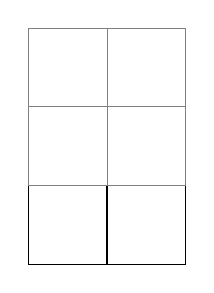
\begin{tikzpicture}[baseline=(current bounding box.east)]
  \draw (0,0) grid (2,1);
  \draw [help lines](0,1) grid (2,3);
\end{tikzpicture}
&
\begin{tikzcode}{}
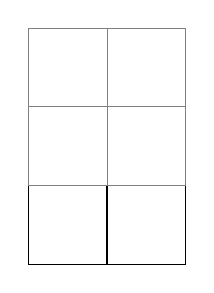
\begin{tikzpicture}
  \draw (0,0) grid (2,1);
  \draw [help lines](0,1) grid (2,3);
\end{tikzpicture}
\end{tikzcode}
\end{tabular}

点命令也非常好理解。其中\verb+\coordinate+是真正将点的名字和坐标联系起来的命令(相当于``赋值''),而\verb+\node+命令仅是一个标注文本的作用。

注意到第二行\verb+\node+命令,它使得字母B标注在pB点315度的位置。这样的效果往往优于其上一行的\verb+\node+命令的效果。注意:\RED{不要忘记{\texttt{\char92{}node}}命令后面的花括号(即使它是空的)}!

\noindent\begin{tabular}{p{0.25\linewidth}l}
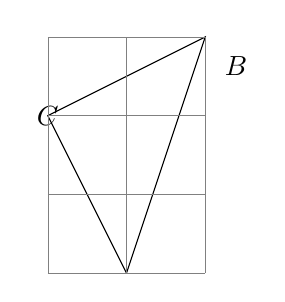
\begin{tikzpicture}[baseline=(current bounding box.east)]
  \coordinate (pA) at (1,0);
  \coordinate (pB) at (2,3);
  \coordinate (pC) at (0,2);
  \node at (pC) {$C$};
  \node[label=315:$B$] at (pB){};
  \draw (pA) -- (pB) -- (pC) -- (pA);
  \draw [help lines](0,0) grid (2,3);
\end{tikzpicture}
&
\begin{tikzcode}{}
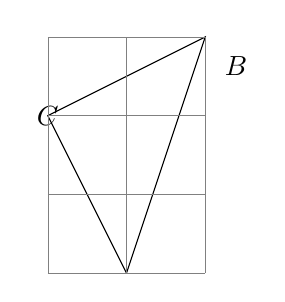
\begin{tikzpicture}
  \coordinate (pA) at (1,0);
  \coordinate (pB) at (2,3);
  \coordinate (pC) at (0,2);
  \node at (pC) {$C$};
  \node[label=315:$B$] at (pB){}; 
  \draw (pA) -- (pB) -- (pC) -- (pA);
  \draw [help lines](0,0) grid (2,3);
\end{tikzpicture}
\end{tikzcode}
\end{tabular}

\subsection{拉伸}
拉伸只需要在tikzpicture后添加xscale/yscale/scale的可选参数赋值即可。例如:

\noindent\begin{tabular}{p{0.25\linewidth}l}
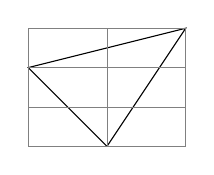
\begin{tikzpicture}[baseline=(current bounding box.east),yscale=0.5]
  \coordinate (pA) at (1,0);
  \coordinate (pB) at (2,3);
  \coordinate (pC) at (0,2);
  \draw (pA) -- (pB) -- (pC) -- (pA);
  \draw [help lines](0,0) grid (2,3);
\end{tikzpicture}
&
\begin{tikzcode}{}
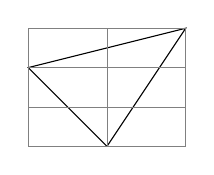
\begin{tikzpicture}[yscale=0.5]
  \coordinate (pA) at (1,0);
  \coordinate (pB) at (2,3);
  \coordinate (pC) at (0,2);
  \draw (pA) -- (pB) -- (pC) -- (pA);
  \draw [help lines](0,0) grid (2,3);
\end{tikzpicture}
\end{tikzcode}
\end{tabular}

\subsection{线宽}
线宽可以在tikzpicture后使用``[line width=5pt]''之类的参数进行\RED{全局调整},也可以在每个draw指令下分别地进行调整:

\noindent\begin{tabular}{p{0.25\linewidth}l}
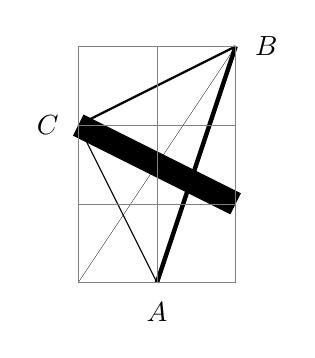
\begin{tikzpicture}[baseline=(current bounding box.east)]
  \coordinate (pA) at (1,0);
  \coordinate (pB) at (2,3);
  \coordinate (pC) at (0,2);
  \node[label=270:$A$] at (pA){};
  \node[label=0:$B$] at (pB){};
  \node[label=180:$C$] at (pC){};
  \draw[ultra thick] (pA) -- (pB);
  \draw[thick] (pB)-- (pC);
  \draw[thin] (pC)-- (pA);
  \draw[ultra thin] (pB) -- (0,0);
  \draw[line width=0.3cm] (pC) -- (2,1);
  \draw [help lines](0,0) grid (2,3);
\end{tikzpicture}
&
\begin{tikzcode}{}
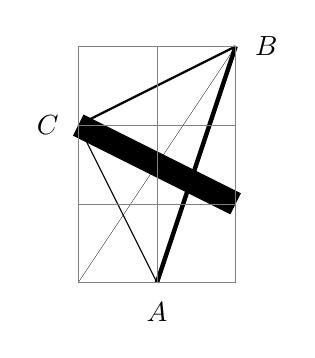
\begin{tikzpicture}
  \coordinate (pA) at (1,0);
  \coordinate (pB) at (2,3);
  \coordinate (pC) at (0,2);
  \node[label=270:$A$] at (pA){};
  \node[label=0:$B$] at (pB){};
  \node[label=180:$C$] at (pC){};
  \draw[ultra thick] (pA) -- (pB);
  \draw[thick] (pB)-- (pC);
  \draw[thin] (pC)-- (pA);
  \draw[ultra thin] (pB) -- (0,0);
  \draw[line width=0.3cm] (pC) -- (2,1);
  \draw [help lines](0,0) grid (2,3);
\end{tikzpicture}
\end{tikzcode}
\end{tabular}

\subsection{填色}
填色的逻辑非常简单,是指向绘制的\qd{闭合}图形内部填色。本例中,draw命令首尾相接地连接三个点,构成一个闭合图形——三角形,因此可以填色:

\noindent\begin{tabular}{p{0.25\linewidth}l}
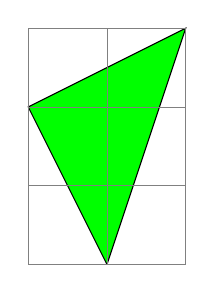
\begin{tikzpicture}[baseline=(current bounding box.east)]
  \coordinate (pA) at (1,0);
  \coordinate (pB) at (2,3);
  \coordinate (pC) at (0,2);
  \draw[fill=green] (pA) -- (pB) -- (pC) -- (pA);
  \draw[help lines](0,0) grid (2,3);
\end{tikzpicture}
&
\begin{tikzcode}{}
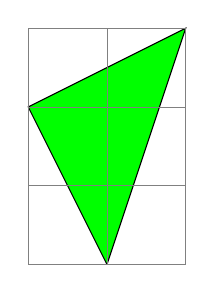
\begin{tikzpicture}
  \coordinate (pA) at (1,0);
  \coordinate (pB) at (2,3);
  \coordinate (pC) at (0,2);
  \draw[fill=green] (pA) -- (pB) -- (pC) -- (pA);
  \draw[help lines] (0,0) grid (2,3);
\end{tikzpicture}
\end{tikzcode}
\end{tabular}

\subsection{点样式}
填色之后图形好看了许多,但是还不够。点标在图中似乎也不看清位置,不过这是有方法解决的:

\noindent\begin{tabular}{p{0.25\linewidth}l}
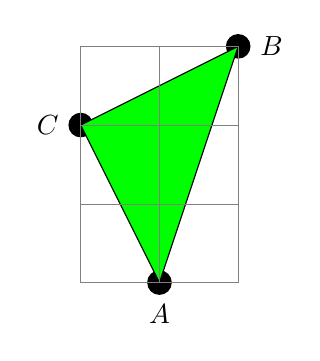
\begin{tikzpicture}[baseline=(current bounding box.east)]
  \coordinate (pA) at (1,0);
  \coordinate (pB) at (2,3);
  \coordinate (pC) at (0,2);
  \node[label=270:$A$,circle,draw,fill,inner sep=3pt] at (pA){};
  \node[label=0:$B$,circle,draw,fill,inner sep=3pt] at (pB){};
  \node[label=180:$C$,circle,draw,fill,inner sep=3pt] at (pC){};
  \draw[fill=green] (pA) -- (pB) -- (pC) -- (pA);
  \draw[help lines] (0,0) grid (2,3);
\end{tikzpicture}
&
\begin{tikzcode}{}
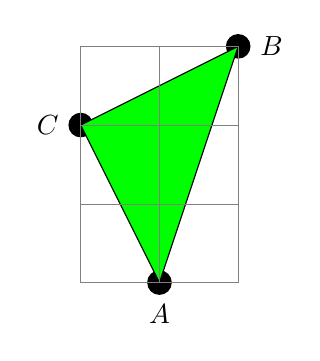
\begin{tikzpicture}
  \coordinate (pA) at (1,0);
  \coordinate (pB) at (2,3);
  \coordinate (pC) at (0,2);
  \node[label=270:$A$,circle,draw,fill,inner sep=3pt] at (pA){};
  \node[label=0:$B$,circle,draw,fill,inner sep=3pt] at (pB){};
  \node[label=180:$C$,circle,draw,fill,inner sep=3pt] at (pC){};
  \draw[fill=green] (pA) -- (pB) -- (pC) -- (pA);
  \draw[help lines] (0,0) grid (2,3);
\end{tikzpicture}
\end{tikzcode}
\end{tabular}

但是这一长串简直是太复杂了。大概能看懂circle是将点画成圆形,fill表示填充,inner sep表示点的大小。而Tikz给出的\verb+\tikzstyle+能够简化步骤。

还有一点就是,绿色的填充似乎位于点的上方?还是乖乖地调整语句顺序吧。

\noindent\begin{tabular}{p{0.25\linewidth}l}
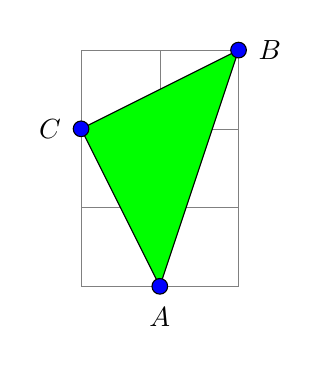
\begin{tikzpicture}[baseline=(current bounding box.east)]
  \draw[help lines] (0,0) grid (2,3);
  \coordinate (pA) at (1,0);
  \coordinate (pB) at (2,3);
  \coordinate (pC) at (0,2);
  \draw[fill=green] (pA) -- (pB) -- (pC) -- (pA);
  \tikzstyle{every node} = [circle,draw,fill=blue,inner sep=2pt];
  \node[label=270:$A$] at (pA){};
  \node[label=0:$B$] at (pB){};
  \node[label=180:$C$] at (pC){};   
\end{tikzpicture}
&
\begin{tikzcode}{}
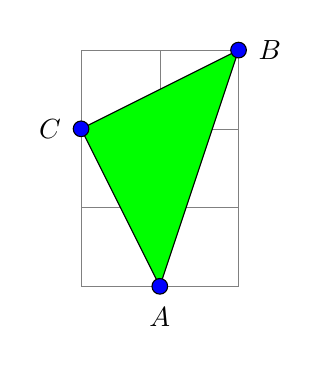
\begin{tikzpicture}
  \draw[help lines] (0,0) grid (2,3);
  \coordinate (pA) at (1,0);
  \coordinate (pB) at (2,3);
  \coordinate (pC) at (0,2);
  \draw[fill=green] (pA) -- (pB) -- (pC) -- (pA);
  \tikzstyle{every node} = [circle,draw,fill=blue,inner sep=2pt];
  \node[label=270:$A$] at (pA){};
  \node[label=0:$B$] at (pB){};
  \node[label=180:$C$] at (pC){}; 
\end{tikzpicture}
\end{tikzcode}
\end{tabular}

注意:\verb+\tikzstyle{every node}+控制的是其下方代码的所有node的点样式,不影响其上方代码中的点。

\subsection{线型和颜色}
除了点的定义,线当然也可以定义。线型有dashed/dotted两种,颜色除了默认的也可以通过叹号的形式控制。

\noindent\begin{tabular}{p{0.25\linewidth}l}
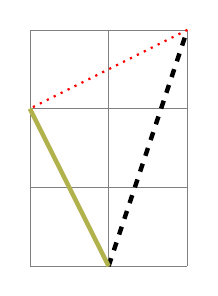
\begin{tikzpicture}[baseline=(current bounding box.east)]
  \draw[help lines] (0,0) grid (2,3);
  \coordinate (pA) at (1,0);
  \coordinate (pB) at (2,3);
  \coordinate (pC) at (0,2);
  \draw[dashed, ultra thick] (pA) -- (pB);
  \draw[dotted, red, thick] (pB) -- (pC);
  \draw[blue!30!yellow, ultra thick] (pC) -- (pA);
\end{tikzpicture}
&
\begin{tikzcode}{}
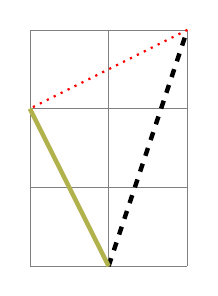
\begin{tikzpicture}
  \draw[help lines] (0,0) grid (2,3);
  \coordinate (pA) at (1,0);
  \coordinate (pB) at (2,3);
  \coordinate (pC) at (0,2);
  \draw[dashed, ultra thick] (pA) -- (pB);
  \draw[dotted, red, thick] (pB) -- (pC);
  \draw[blue!30!yellow, ultra thick] (pC) -- (pA);
\end{tikzpicture}
\end{tikzcode}
\end{tabular}

主要的颜色包括\footnote{以下色块用\texttt{\char92{}tikz\{\char92{}draw[{\it color},line width=9] (0,0) -- (0.5,0);\}绘制得到。}}:
\tikzline{red}\tikzline{green}\tikzline{yellow}\tikzline{blue}\tikzline{cyan}
\tikzline{magenta}\tikzline{black}\tikzline{gray}\tikzline{darkgray}\tikzline{lightgray}
\tikzline{brown}\tikzline{lime}\tikzline{olive}\tikzline{orange}\tikzline{pink}\tikzline{purple}
\tikzline{teal}\tikzline{violet}
还有white\tikz{\draw[white,line width=9](0,0)--(0.5,0);}.

\subsection{箭头}
箭头也是需要经常绘制的内容。主要也是根据\verb+\draw+命令的参数控制:

\noindent\begin{tabular}{p{0.25\linewidth}l}
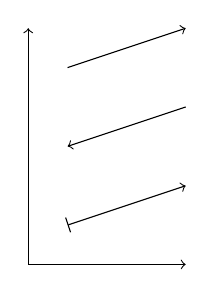
\begin{tikzpicture}[baseline=(current bounding box.east)]
  \draw[->] (0.5,2.5) -- (2,3);
  \draw[<-] (0.5,1.5) -- (2,2);
  \draw[|->] (0.5,0.5)-- (2,1); 
  \draw[<->] (0,3) -- (0,0) -- (2,0);
\end{tikzpicture}
&
\begin{tikzcode}{}
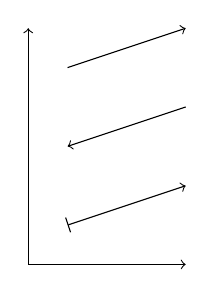
\begin{tikzpicture}
  \draw[->] (0.5,2.5) -- (2,3);
  \draw[<-] (0.5,1.5) -- (2,2);
  \draw[|->] (0.5,0.5)-- (2,1); 
  \draw[<->] (0,3) -- (0,0) -- (2,0);
\end{tikzpicture}
\end{tikzcode}
\end{tabular}

\section{高效书写}
\subsection{变量}
变量申请使用与\LaTeX 相同的语句:\verb+\newcommand+. 注意:变量需要以反斜杠开头,并与现有命令不重复。

\noindent\begin{tabular}{p{0.25\linewidth}l}
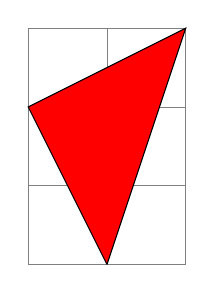
\begin{tikzpicture}[baseline=(current bounding box.east)]
  \draw [help lines](0,0) grid (2,3);
  \newcommand{\aaa}{1};
  \newcommand{\bbb}{3};
  \newcommand{\ccc}{2};
  \coordinate (pA) at (\aaa,0);
  \coordinate (pB) at (\ccc,\bbb);
  \coordinate (pC) at (0,\ccc);
  \draw[fill=red] (pA) -- (pB) -- (pC) -- (pA); 
\end{tikzpicture}
&
\begin{tikzcode}{}
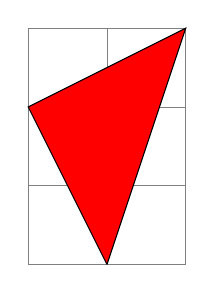
\begin{tikzpicture}
  \draw [help lines](0,0) grid (2,3);
  \newcommand{\aaa}{1};
  \newcommand{\bbb}{3};
  \newcommand{\ccc}{2};
  \coordinate (pA) at (\aaa,0);
  \coordinate (pB) at (\ccc,\bbb);
  \coordinate (pC) at (0,\ccc);
  \draw[fill=red] (pA) -- (pB) -- (pC) -- (pA); 
\end{tikzpicture}
\end{tikzcode}
\end{tabular}

\subsection{循环}
但是同样的语句书写很多遍是很复杂的,好在Tikz提供了循环的实现方法:

\noindent\begin{tabular}{p{0.25\linewidth}l}
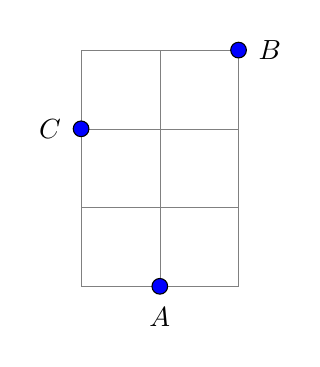
\begin{tikzpicture}[baseline=(current bounding box.east)]
  \newcommand{\la}{1};
  \newcommand{\lb}{3};
  \newcommand{\lc}{2};
  \draw [help lines](0,0) grid (\lc,\lb);
  \coordinate (pA) at (\la,0);
  \coordinate (pB) at (\lc,\lb);
  \coordinate (pC) at (0,\lc);
  \tikzstyle{every node}=[circle, draw, fill=blue,inner sep=2pt];
  \foreach \x/\y in {A/270,B/0,C/180}{
    \node[label=\y:$\x$] at (p\x){};
  }
\end{tikzpicture}
&
\begin{tikzcode}{}
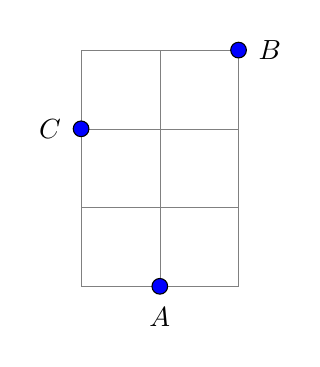
\begin{tikzpicture}
  \newcommand{\la}{1};
  \newcommand{\lb}{3};
  \newcommand{\lc}{2};
  \draw [help lines](0,0) grid (\lc,\lb);
  \coordinate (pA) at (\la,0);
  \coordinate (pB) at (\lc,\lb);
  \coordinate (pC) at (0,\lc);
  \tikzstyle{every node}=[circle, draw, fill=blue,inner sep=2pt];
  \foreach \x/\y in {A/270,B/0,C/180}{
    \node[label=\y:$\x$] at (p\x){};
  }
\end{tikzpicture}
\end{tikzcode}
\end{tabular}

注意到:甚至点的名称pA, pB, pC中的A, B, C也是可以通过foreach来指定的!

\subsection{运算}
\fbox{{\itshape{注意:需要在导言区添加}}\latexline{\\usetikzlibrary{calc}}。文中不再写出。}

如果一个绘图工具仅仅能够绘图而不能做运算……它有什么用呢?如果作为科学排版系统下的绘图工具而不支持运算的话,Tikz岂不是太弱了?

\noindent\begin{tabular}{p{0.25\linewidth}l}
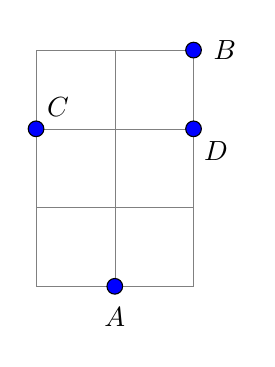
\begin{tikzpicture}[baseline=(current bounding box.east)]
  \draw [help lines](0,0) grid (2,3);
  \coordinate (pA) at (1,0);
  \coordinate (pB) at (2,3);
  \coordinate (pC) at (0,2);
  \coordinate (pD) at ($(pB)+(0,-1)$);
  \tikzstyle{every node}=[circle, draw, fill=blue,inner sep=2pt];
  \foreach \x/\y in {A/270,B/0,C/45,D/315}{
    \node[label=\y:$\x$] at (p\x){};
  }
\end{tikzpicture}
&
\begin{tikzcode}{}
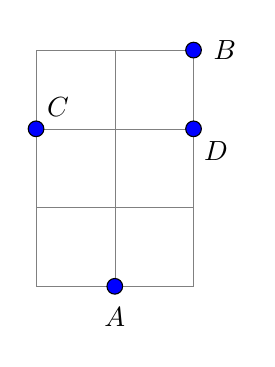
\begin{tikzpicture}
  \draw [help lines](0,0) grid (2,3);
  \coordinate (pA) at (1,0);
  \coordinate (pB) at (2,3);
  \coordinate (pC) at (0,2);
  \coordinate (pD) at ($(pB)+(0,-1)$);
  \tikzstyle{every node}=[circle, draw, fill=blue,inner sep=2pt];
  \foreach \x/\y in {A/270,B/0,C/45,D/315}{
    \node[label=\y:$\x$] at (p\x){};
  }
\end{tikzpicture}
\end{tikzcode}
\end{tabular}

\clearpage
\begin{appendices}
\renewcommand{\thechapter}{\Alph{chapter}}
\titleformat{\chapter}[display]{\Huge\bfseries}{附录\Alph{chapter}}{1em}{}
%\renewcommand{\thesection}{\thechapter-\arabic{section}}
%\titleformat{\section}[hang]{\bfseries\Large}{\S\ \thesection}{1em}{}{}

\chapter{注音符号}
\label{app:phonetic}
% 这里不用>{\ttfamily}而用\verb是为了减少报错可能
\begin{center}
\tabcaption{注音符号与特殊符号}
\begin{tabular}{|*{4}{>{\centering}p{4em} @{-\hspace{1em}} p{3em}|}}
\hline
\texttt{样式} & 命令 & \texttt{样式} & 命令 & \texttt{样式} & 命令 & \texttt{样式} & 命令 \\
\hline
\=o  & \verb|\=o|  & \'o  & \verb|\'o|  & \v o & \verb|\v o|  & \`o   & \verb|\`o|  \\
\^o  & \verb|\^o|  & \"o  & \verb|\"o|  & \.o  & \verb|\.o|   & \H o  & \verb|\H o| \\
\d o & \verb|\d o| & \u o & \verb|\u o| & \b o & \verb|\b o|  & \t oo & \verb|\t oo|\\
\multicolumn{2}{|c@{\bf --}}{$\tilde{o}$} & \multicolumn{2}{@{\bf --}c|}{\tt{\$$\backslash$tilde\{o\}\$}} &%
\multicolumn{2}{c@{\bf --}}{$\hat{o}$}    & \multicolumn{2}{@{\bf --}c|}{\tt{\$$\backslash$hat\{o\}\$}}\\
& & & & & & & \\
\o  & \verb|\o|  & \O  & \verb|\O|  & \i  & \verb|\i|  & \j  & \verb|\j| \\
\aa & \verb|\aa| & \AA & \verb|\AA| & \ae & \verb|\ae| & \AE & \verb|\AE|\\
\oe & \verb|\oe| & \OE & \verb|\OE| & !`  & \verb|!`|  & ?`  & \verb|?`| \\
\hline
\end{tabular}
\end{center}

\mbox{}

\begin{center}
\tabcaption{国际音标输入表(部分)}
\begin{tabular}{|*{3}{>{\centering\rmfamily}p{3em} @{-\hspace{0.5em}} >{\ttfamily}p{7.5em}|}}
\hline
\texttt{样式} & 命令 & \texttt{样式} & 命令 & \texttt{样式} & 命令 \\
\hline
\textdzlig & \char92textdzlig & \textesh & \char92textesh & \textteshlig & \char92textteshlig \\
\textdyoghlig & \char92textdyoghlig & \textturnv & \char92textturnv & \textschwa & \char92textschwa \\
\textscriptg & \char92textscriptg & \texttheta & \char92texttheta & \textupsilon & \char92textupsilon \\
\textscripta & \char92textscripta & \dh & \char92dh & \textepsilon & \char92textepsilon \\
\textopeno & \char92textopeno & \textyogh & \char92textyogh & \ng & \char92ng \\
\hline
\multicolumn{2}{|c|}{重音} & \multicolumn{2}{c|}{次重音} & \multicolumn{2}{c|}{长音节} \\
\textprimstress & \char92{}textprimstress & \textsecstress & \char92textsecstress & \textlengthmark & \char92textlengthmark \\
\hline
\end{tabular}
\end{center}

\textit{注:\texttt{\char92dh}命令在非CJK文档中有时编译会出现问题}。

\end{appendices}

\end{document}
